\documentclass[a4paper, 12pt]{extarticle}

\usepackage{xecyr}
\usepackage{color}
\usepackage{float}
\usepackage{fontenc}
\usepackage{amsmath}
\usepackage{xltxtra}
\usepackage{graphicx}
\usepackage{csquotes}
\usepackage{listings}
\usepackage{longtable}
\usepackage{indentfirst}
\usepackage{unicode-math}
\usepackage{subfig}
\usepackage[english, russian]{babel}
\usepackage[width=1.2\textwidth]{caption}

\usepackage{titlesec}
\titleformat{\section}
  {\normalfont\fontsize{14}{15}\bfseries}{\thesection.}{5pt}{}
\titleformat{\subsection}
  {\normalfont\fontsize{14}{15}\bfseries}{\thesubsection.}{5pt}{}
\titleformat{\subsubsection}
  {\normalfont\fontsize{14}{15}\bfseries}{\thesubsubsection.}{5pt}{}

\usepackage{fontspec}
\defaultfontfeatures{Ligatures=TeX}
\setmainfont[Ligatures=TeX]{Times New Roman}

\usepackage[a4paper,margin=1in,heightrounded]{geometry}
\geometry{left=2.5cm}
\geometry{right=1.5cm}
\geometry{top=2cm}
\geometry{bottom=2cm}

\usepackage{expl3}
\ExplSyntaxOn
\cs_new_eq:NN \Repeat \prg_replicate:nn
\ExplSyntaxOff

\usepackage[maxnames=5,
        backend=biber,
        style=gost-numeric,
        sorting=none,
        autolang=other]{biblatex}
\addbibresource{bibliography.bib}

% Sections style redefinition
\renewcommand{\thesection}
  {\thepart\arabic{section}}
\renewcommand{\thesubsection}
  {\thepart\arabic{section}.\arabic{subsection}}
\renewcommand{\thesubsubsection}
  {\thepart\arabic{section}.\arabic{subsection}.\arabic{subsubsection}}


% Equations, fugures, tables numbering style redefinition
\renewcommand{\theequation}
  {\thesection.\arabic{equation}}
\renewcommand{\thefigure}
  {\thesection.\arabic{figure}}
\renewcommand{\thetable}
  {\thesection.\arabic{table}}

% Enum style redefinition
\renewcommand{\labelenumii}
  {\labelenumi\arabic{enumii}.}
\renewcommand{\labelenumiii}
  {\labelenumii\arabic{enumiii}.}

% Enlarge table row height
\renewcommand{\arraystretch}{1.2}

% Font to inline code highlighting
% Consolas must be installed!!!
\newfontfamily{\codefont}[Scale=0.9]{Consolas}
\newfontfamily{\listingsfont}[Scale=1.0]{Consolas}

% Define default style for codelisitngs
\definecolor{codegreen}{rgb}{0.00, 0.50, 0.00}
\definecolor{codegray} {rgb}{0.50, 0.50, 0.50}
\definecolor{codenumb} {rgb}{0.00, 0.00, 1.00}
\definecolor{codeblue} {rgb}{0.00, 0.43, 0.13}
\definecolor{codebrick}{rgb}{0.64, 0.08, 0.08}
\lstset{
  backgroundcolor=\color{white},
  basicstyle=\fontsize{10}{12}\selectfont\listingsfont,
  breakatwhitespace=false,
  breaklines=true,
  captionpos=b,
  commentstyle=\color{codegreen},
  frame=l,
  keepspaces=true,
  keywordstyle=\color{codeblue},
  language=C++,
  numbers=left,
  numbersep=8pt,
  numberstyle=\tiny\color{codegray},
  rulecolor=\color{black},
  showspaces=false,
  showstringspaces=false,
  showtabs=false,
  stepnumber=1,
  stringstyle=\color{codebrick},
  tabsize=2,
  title=\lstname
}

% Listing numbering style redefinition
\renewcommand{\lstlistingname}{Листинг}
\AtBeginDocument{
  \renewcommand{\thelstlisting}{\thesection\arabic{lstlisting}}
}

\newtheorem{hypothesis}{Гепотеза}
\newtheorem{theorem}{Теорема}

\DeclareMathOperator*{\argmax}{arg\,max}
\DeclareMathOperator*{\argmin}{arg\,min}
\DeclareMathOperator{\sign}{sign}
\DeclareMathOperator{\re}{\operatorname{Re}}

\begin{document}

\begingroup
\fontsize{14pt}{17pt}\selectfont
\begin{titlepage}

\begin{center}
МИНИСТЕРСТВО ОБРАЗОВАНИЯ И НАУКИ РОССИЙСКОЙ ФЕДЕРАЦИИ \\*
Федеральное   государственное  автономное  образовательное  учреждение \\*
высшего образования \\*
\textbf{<<Национальный исследовательский \\*
Нижегородский государственный университет им. Н.И. Лобачевского>> \\*
(ННГУ)}
\end{center}

\vspace{12pt}

\begin{center}
\textbf{Институт информационных технологий, математики и механики}
\end{center}

\begin{center}
\textbf{Кафедра: Математического обеспечения и суперкомпьютерных технологий}
\end{center}

\vspace{25pt}
\begin{center}
Направление подготовки: «Прикладная математика и информатика» \\*
Магистерская программа: «Системное программирование»
\end{center}
\vspace{30pt}

\begin{center}
\fontsize{18pt}{0pt}\textbf{ОТЧЁТ} \\*
по преддипломной практике
\end{center}
\begin{center}
на тему: \\*
\fontsize{16pt}{0pt}\textbf{<<Разработка эффективных структурх хранения данных для алгоритмов глобальной оптимизации>>}
\end{center}

\vspace{53pt}

\begin{flushright}
\textbf{Выполнил}: студент группы 381503м4 \\*
\Repeat{17}{\_} Соврасов В.В. \\*
Подпись \Repeat{32}{\ } \\*

\textbf{Научный руководитель}: \Repeat{21}{\ } \\*
доцент, к.ф.м.н. \Repeat{36}{\ } \\*
\Repeat{17}{\_} Баркалов К.А. \\*
Подпись \Repeat{32}{\ }
\end{flushright}

\vspace{\fill}

\begin{center}
Нижний Новгород \\*
2017
\end{center}

\end{titlepage}
 % Link to main page
\endgroup

\begingroup
\fontsize{12pt}{20pt}\selectfont

\newpage
\thispagestyle{empty}
\tableofcontents

\newpage
\setcounter{page}{1}
\section{Введение}
Задачи нелинейной глобальной оптимизации встречаются в различных прикладных областях и
традиционно считаются одними из самых трудоёмких среди оптимизационных задач.
Их сложность экспоненциально растёт в зависимости от размерности пространства поиска,
поэтому для решения существенно многомерных задач требуются суперкомпьютерные вычисления.

В настоящее время на кафедре МОиСТ активно ведётся разработка программной системы
для глобальной оптимизации функций многих вещественных переменных Globalizer.
Эта система включает в себя последние теоретические разработки, сделанные на кафедре в
этой сфере, в том числе и блочную многошаговую схему редукции размерности \cite{blockNested}.
Отличительной чертой ситемы является то, что, она может работать как на CPU, так на
разных типах ускорителей вычислений с высокой степенью параллельности (XeonPhi, GPU Nvidia) \cite{examinArtcle, examinphiArtcle}.

В данной работе будут описаны некеторые улучшения, внесённые в систему, и предварительные исследования, проведённые перед их внедрением.

\section{Постановка задачи глобальной липшицевой оптимизации}
Одна из постановок задачи глобальной оптимизации звучит следующим образом: найти
глобальный минимум \(N\)-мерной функции \(\varphi(y)\) в гиперинтервале
\(D=\{y\in R^N:a_i\leqslant x_i\leqslant{b_i}, 1\leqslant{i}\leqslant{N}\}\).
Для построения оценки глобального минимума по конечному количеству вычислений
значения функции требуется, чтобы \(\varphi(y)\) удовлетворяла условию Липшица.
\begin{displaymath}
\label{task}
\varphi(y^*)=\min\{\varphi(y):y\in D\}
\end{displaymath}
\begin{displaymath}
\label{lip}
|\varphi(y_1)-\varphi(y_2)|\leqslant L\Vert y_1-y_2\Vert,y_1,y_2\in D,0<L<\infty
\end{displaymath}

Классической схемой редукции размерности для алгоритмов глобальной оптимизации является
использование разверток --- кривых, заполняющих пространство \cite{strOptBook}.
\begin{displaymath}
\label{cube}
\lbrace y\in R^N:-2^{-1}\leqslant y_i\leqslant 2^{-1},1\leqslant i\leqslant N\rbrace=\{y(x):0\leqslant x\leqslant 1\}
\end{displaymath}
На рис. \ref{fig:peano_curve} представлены построенные численно с низкой точностью развёртки на плоскости и
в трёхмерном пространстве.

\begin{figure}[ht]
    \centering
    \subfloat{{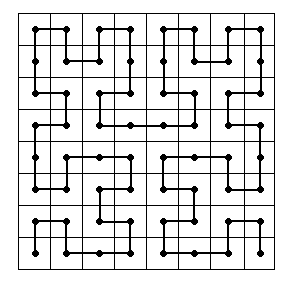
\includegraphics[width=0.45\textwidth]{images/peano2d.png} }}
    \qquad
    \subfloat{{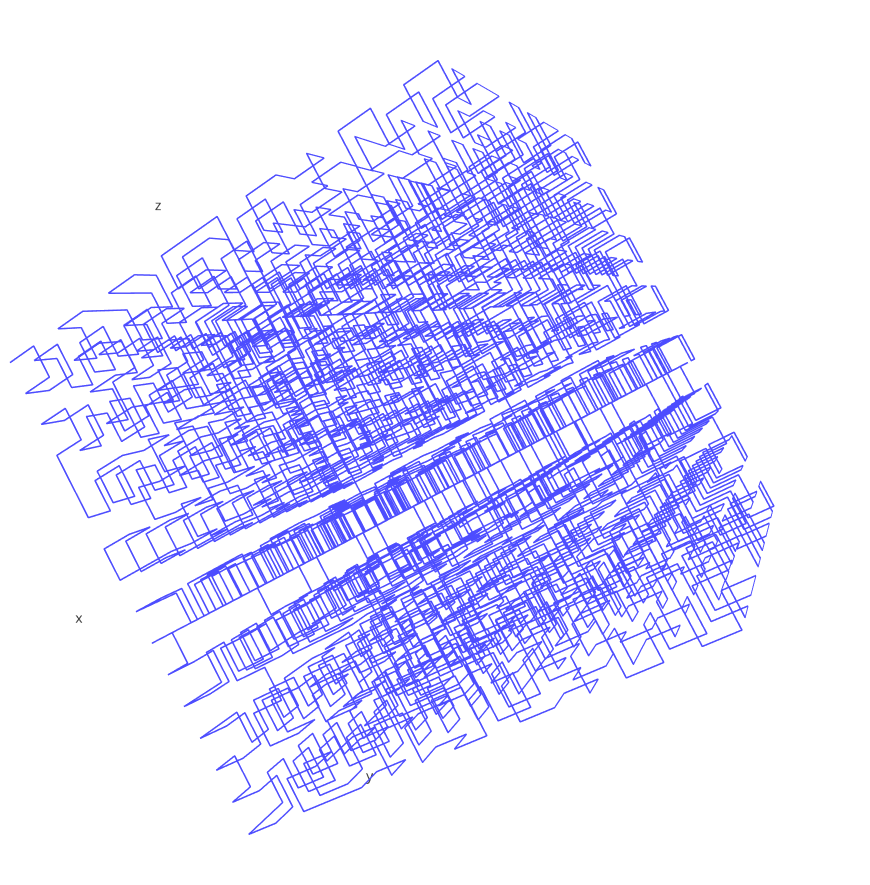
\includegraphics[width=0.45\textwidth]{images/peano3d.png} }}
    \caption{Численно построенная развёртка в двухмерном и трёхмерном случаях}
    \label{fig:peano_curve}
\end{figure}

Такое отображение позволяет свести задачу в многомерном пространстве к решению
одномерной ценой ухудшения её свойств. В частности, одномерная функция \(\varphi(y(x))\)
является не Липшицевой, а Гёльдеровой:
\begin{displaymath}
\label{holder}
|\varphi(y(x_1))-\varphi(y(x_2))|\leqslant H{|x_1-x_2|}^{\frac{1}{N}},x_1,x_2\in[0;1],
\end{displaymath}
где константа Гельдера \(H\) связана с константой Липшица \(L\) соотношением
\begin{displaymath}
H=4Ld\sqrt{N},d=\max\{b_i-a_i:1\leqslant i\leqslant N\}.
\end{displaymath}
На рис. \ref{fig:evolvent_example} приведена одномерная функция, полученная после применения развёртки к
парабалоиду вращения \(\varphi(y)=y_1^2+y_2^2\).

\begin{figure}[ht]
    \center
    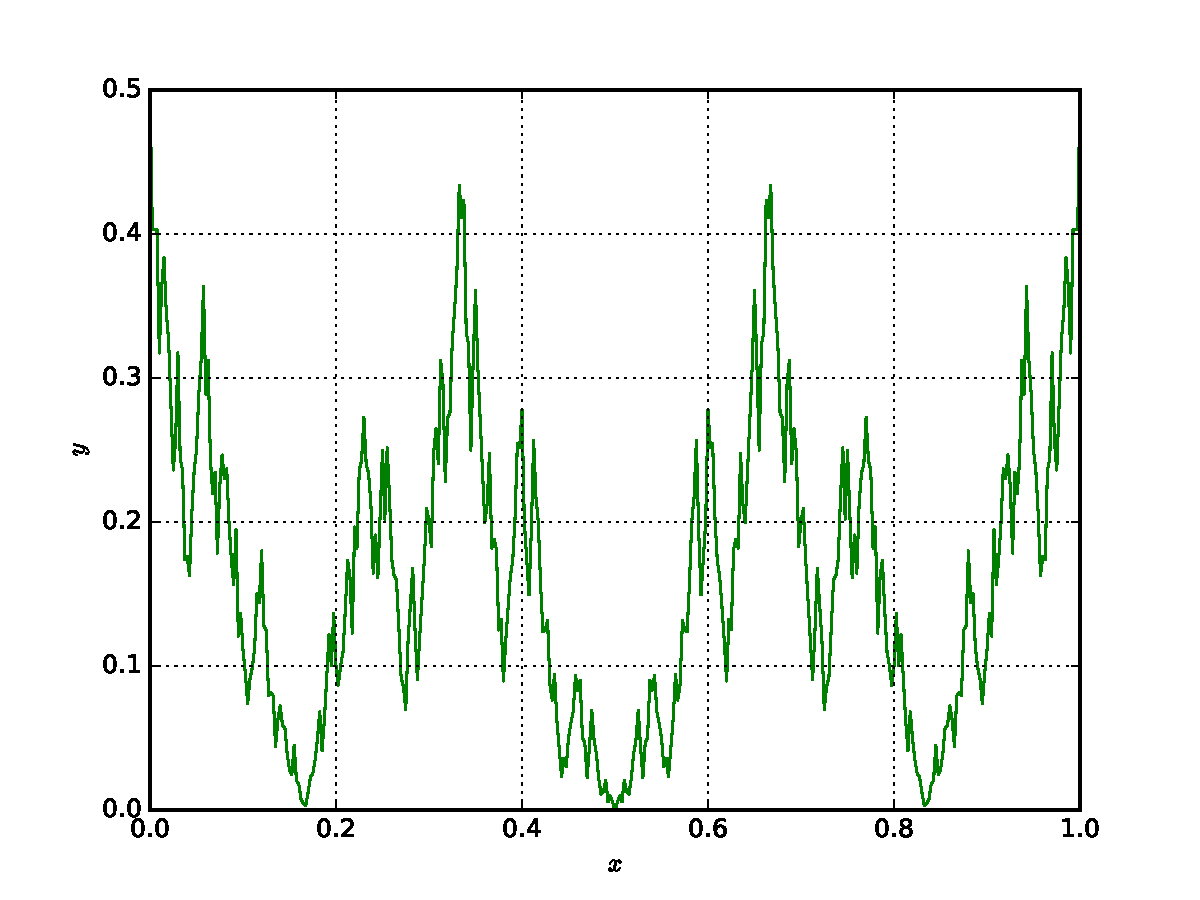
\includegraphics[width=0.75\textwidth]{images/map_paraboloid.pdf}
    \caption{Пример одномерной функции, порождённой развёрткой}
    \label{fig:evolvent_example}
\end{figure}

Область \(D\) также может быть задана с помощью функциональных ограничений.
Постановка задачи глобальной оптимизации в этом случае будет иметь следующий вид:
\begin{equation}
  \label{eq:constrained_problem}
  \varphi(y^*)=\min\{\varphi(y):g_j(y)\leqslant 0, 1\leqslant j\leqslant m\}
\end{equation}
Обозначим \(g_{m+1}(y)=f(y)\). Далее будем предполагать, что все функции \(g_k(y),1\leqslant k \leqslant m+1\)
удовлетворяют условию Липшица в некотором гиперинтервале, включающем \(D\).

\section{Алгоритм глобального поиска} \label{sec:method}
Для дальнейшего изложения потребуется описание метода глобальной оптимизации,
используемого в системе Globalizer. Многомерные задачи сводятся к одномерным с помощью
различных схем редукции размерности, поэтому можно рассматривать минимизацию одномерной
функции \(f(x), x\in[0;1]\), удовлетворяющей условию Гёльдера, при ограничениях, также
удовлетворяющих этому условию на интервале \([0;1]\).

Рассматриваемый алгоритм решения одномерной задачи (\ref{eq:constrained_problem}) предполагает построение последовательности
точек \(x_k\), в которых вычисляются значения минимизируемой функции или ограничений \(z_k = g_s(x_k)\).
Для учёта последних используется индексная схема \cite{strongSerg}. Пусть \(Q_0=[0;1]\). Ограничение, имеющее номер
 \(j\), выполняется во всех точках области
\begin{displaymath}
  Q_j=\left\{x\in [0;1]:g_j(x)\leq 0\right\},
\end{displaymath}
которая называется допустимой для этого ограничения. При этом допустимая область \(D\)
исходной задачи определяется равенством: \(D=\cap _{j=0}^{m}Q_{j}\).
Испытание в точке \(x\in [0;1]\) состоит в последовательном вычислении значений
величин \(g_{1}(x),...,g_{\nu }(x)\), где значение индекса \(\nu\) определяется условиями:
\(x\in Q_{j},0\leqslant j<\nu ,x\notin Q_{\nu }\). Выявление первого нарушенного ограничения
прерывает испытание в точке \(x\). В случае, когда точка \(x\)  допустима, т. е.
\(x\in D\) испытание включает в себя вычисление всех функций задачи. При этом значение
индекса принимается равным величине \(\nu =m+1\). Пара \(\nu =\nu (x),z=g_{\nu }(x)\),
где индекс \(\nu\) лежит в границах \(1\leqslant \nu \leqslant m+1\), называется результатом
испытания в точке \(x\).

Такой подход к проведению испытаний позволяет свести исходную задачу с функциональными
ограничениями к безусловной задаче минимизации разрывной функции:

\begin{displaymath}
  \begin{array}{lr}
    \psi (x^{*})=\min_{x\in [0;1]}\psi (x), \\
    \psi (x)={\begin{cases}g_{\nu }(x)/H_{\nu }&\nu <M\\(g_{M}(x)-g_{M}^{*})/H_{M}&\nu =M\end{cases}}
  \end{array}
\end{displaymath}

Здесь \(M=\max_{}^{}\left\{\nu (x):x\in [0;1]\right\}\), а \(g_{M}^{*}=\min _{}^{}\left\{g_{M}(x):x\in \cap _{i=0}^{M-1}Q_{i}\right\}\).
В силу определения числа \(M\), задача отыскания \(g_{M}^{*}\)
всегда имеет решение, а если \(M=m+1\), то \(g_{M}^{*}=f(x^{*})\).
Дуги функции \(\psi (x)\) гельдеровы на множествах \(\cap _{i=0}^{j}Q_{i},0\leq j\leq M-1\)
с константой 1, а сама \(\psi (x)\) может иметь разрывы первого рода на границах этих множеств.
Несмотря на то, что значения констант Гёльдера \(H_k\) и величина \(g_{M}^{*}\) заранее неизвестны,
они могут быть оценены в процессе решения задачи.

Множество троек \(\{(x_k,\nu_k,z_k)\}, 1\leqslant k\leqslant n\) составляет поисковую информацию,
накопленную методом после проведения \(n\) шагов.

На первой итерации метода испытание проводится в произвольной внутренней точке \(x_1\)
интервала \([0;1]\). Индексы точек 0 и 1 считаются нулевыми, значения \(z\) в
них не определены. Пусть выполнено \(k\geqslant 1\) итераций метода,
в процессе которых были проведены испытания в \(k\) точках \(x_i, 1\leqslant i\leqslant k\).
Тогда точкa \(x^{k+1}\) поисковых испытаний следующей \((k+1)\)-ой
итерации определяются в соответствии с правилами:

Шаг 1. Перенумеровать точки множества \(X_k=\{x^1,\dotsc,x^k\}\cup\{0\}\cup\{1\}\),
которое включает в себя граничные точки интервала \([0;1]\), а также точки предшествующих
испытаний, нижними индексами в порядке увеличения значений координаты, т.е.
\begin{displaymath}
0=x_0<x_1<\dotsc<x_{k+1}=1
\end{displaymath}
и сопоставить им значения \(z_{i}=g_{\nu }(x_{i}),\nu =\nu (x_{i}),i={\overline {1,k}}\).

Шаг 2. Для каждого целого числа \(\nu ,1\leqslant \nu \leqslant m+1\) определить соответствующее
ему множество \(I_{\nu }\) нижних индексов точек, в которых вычислялись значения
функций \(g_{\nu }(x)\):
\begin{displaymath}
  I_{\nu }=\{i:\nu (x_{i})=\nu ,1\leqslant i\leqslant k\},1\leq \nu \leqslant m+1,
\end{displaymath}
определить максимальное значение индекса \(M=\max\{\nu (x_{i}),1\leq i\leq k\}\).

Шаг 3. Вычислить текущие оценки для неизвестных констант Гёльдера:
\begin{equation}
  \label{step2}
  \mu _{\nu }=\max\{\frac{|g_{\nu }(x_{i})-g_{\nu }(x_{j})|}{(x_{i}-x_{j})^{\frac{1}{N}}}:i,j\in I_{\nu },i>j\}.
\end{equation}
Если множество \(I_{\nu }\) содержит менее двух элементов или если значение \(\mu _{\nu }\)
оказывается равным нулю, то принять \(\mu _{\nu }=1\).

Шаг 4. Для всех непустых множеств \(I_{\nu },\nu ={\overline {1,M}}\) вычислить оценки
\begin{displaymath}
  z_{\nu }^{*}={\begin{cases}\min\{g_{\nu }(x_{i}):x_{i}\in I_{\nu }\}&\nu =M\\-\varepsilon _{\nu }&\nu <M\end{cases}},
\end{displaymath}
где вектор с неотрицательными координатами \(\varepsilon _{R}=(\varepsilon _{1},..,\varepsilon _{m})\) называется вектором резервов.

Шаг 5. Для каждого интервала \((x_{i-1};x_{i}),1\leqslant i\leqslant k\) вычислить характеристику
\begin{equation}
  \label{step3_1}
  R(i)={\begin{cases}\Delta _{i}+{\frac {(z_{i}-z_{i-1})^{2}}{(r_{\nu }\mu _{\nu })^{2}\Delta _{i}}}-2{\frac {z_{i}+z_{i-1}-2z_{\nu }^{*}}{r_{\nu }\mu _{\nu }}}&\nu =\nu (x_{i})=\nu (x_{i-1})\\2\Delta _{i}-4{\frac {z_{i-1}-z_{\nu }^{*}}{r_{\nu }\mu _{\nu }}}&\nu =\nu (x_{i-1})>\nu (x_{i})\\2\Delta _{i}-4{\frac {z_{i}-z_{\nu }^{*}}{r_{\nu }\mu _{\nu }}}&\nu =\nu (x_{i})>\nu (x_{i-1})\end{cases}}
\end{equation}
где \(\Delta _{i}=(x_{i}-x_{i-1})^{\frac{1}{N}}\). Величины \(r_{\nu }>1,\nu ={\overline {1,m}}\)
являются параметрами алгоритма. От них зависят произведения \(r_{\nu }\mu _{\nu }\),
используемые при вычислении характеристик в качестве оценок неизвестных констант Гёльдера.

Шаг 5. Выбрать наибольшую характеристику:
\begin{equation}
\label{step4}
t=\argmax_{1\leqslant i \leqslant k+1}R(i)
\end{equation}

Шаг 6. Провести очередное испытание в середине интервала \((x_{t-1};x_{t})\),
если индексы его концевых точек не совпадают: \(x^{k+1}={\frac {1}{2}}(x_{t}+x_{t-1})\).
В противном случае провести испытание в точке
\begin{displaymath}
  x^{k+1}={\frac {1}{2}}(x_{t}+x_{t-1})-\operatorname {sgn}(z_{t}-z_{t-1}){\frac {|z_{t}-z_{t-1}|^{n}}{2r_{\nu }\mu _{\nu }^{n}}},\nu =\nu (x_{t})=\nu (x_{t-1}),
\end{displaymath}
а затем увеличить \(k\) на 1.

Алгоритм прекращает работу, если выполняется условие \(\Delta_{t}\leqslant \varepsilon\),
где \(\varepsilon>0\) есть заданная точность. В качестве оценки глобально-оптимального решения задачи  выбираются значения
\begin{equation}
f_k^*=\min_{1\leqslant i \leqslant k}f(x_i), x_k^*=\argmin_{1\leqslant i \leqslant k}f(x_i)
\end{equation}

Достаточные условия сходимости метода определяются следующей теоремой:
\begin{theorem}
  Пусть исходная задача оптимизации имеет решение \(x^{*}\) и выполняются следующие условия:
  \begin{itemize}
    \item каждая область \(Q_{j},j={\overline {1,m}}\) представляет собой объединение
    конечного числа отрезков, имеющих положительную длину;
    \item каждая функция \(g_{j}(x),j={\overline {1,m+1}}\) удовлетворяет условию Гёльдера с соответствующей константой \(H_{j}\);
    \item компоненты вектора резервов удовлетворяют неравенствам \(0\leq 2\varepsilon _{\nu }<L_{\nu }(\beta -\alpha )\),
    где \(\beta -\alpha\) --- длина отрезка \([\alpha ;\beta ]\), лежащего в допустимой области \(D\) и содержащего точку \(x^{*}\);
    \item начиная с некоторого значения \(k\) величины \(\mu _{\nu }\), соответствующие
    непустым множествам \(I_{\nu }\), удовлетворяют неравенствам \(r_{\nu }\mu _{\nu }>2H_{\nu }\).
  \end{itemize}
  Тогда верно следующее:
  \begin{itemize}
    \item точка \(x^{*}\) является предельной точкой последовательности \(\{x^{k}\}\), порождаемой методом при \(\varepsilon =0\)  в условии остановки;
    \item любая предельная точка \(x^{0}\)  последовательности \(\{x^{k}\}\) является решением исходной задачи оптимизации;
    \item сходимость к предельной точке \(x^{0}\) является двухсторонней, если \(x^{0}\not =a,x^{0}\not =b\).
  \end{itemize}
\end{theorem}

Подробнее метод и теорема о его сходимости описаны в \cite{strongSerg}.

\subsection{Сравнение методов оптимизации} \label{subsec:methods_compasion}
Существует несколько критериев оптимальности алгоритмов поиска (минимаксный, критерий
одношаговой оптимальности), но большинстве случаев представляет интерес
сравнение методов по среднему результату, достижимому на конкретном подклассе липшицевых функций.
Достоинством такого подхода является то, что средний показатель можно оценить
по конечной случайной выборке задач, используя методы математической статистики.

В качестве оценки эффективности алгоритма будем использовать, операционную характеристику,
которая определяется множеством точек на плоскости \((K, P)\),
где \(K\) – среднее число поисковых испытаний, предшествующих выполнению условия
остановки при минимизации функции из данного класса, а \(P\) – статистическая вероятность того,
что к моменту остановки глобальный экстремум будет найден с заданной точностью.
Если при выбранном \(K\) операционная характеристика одного метода лежит выше характеристики другого,
то это значит, что при фиксированных затратах на поиск первый метод найдёт решение с
большей статистической вероятностью. Если же зафиксировать некоторое значение \(P\), и
характеристика одного метода лежит левее характеристики другого, то первый метод
требует меньше затрат на достижение той же надёжности.

\subsection{Классы тестовых задач} \label{subsec:test_problems}
Для сравнения алгоритмов глобального поиска в смысле операционной характеристики
требуется иметь некоторое множество тестовых задач. Генератор задач GKLS, описанный в
\cite{gklsBook} позволяет получить такое множество задач с заренее известными свойствами.
Это достигается за счёт модификации параболоида \(g(x)=\Vert x-T\Vert + t\) в
шаровых окрестностях некоторых случайно сгенерированных точек \(M_i, i=\overline{1,m}\). В точках
\(M_i\) распологаются локальные минимумы со значениями, превосходящими значение
\(g(T)=t\). Таким образом, координаты глобального минимума в задачах GKLS всегда заведомо известны.
В данной работе используется несколько классов, сгенерированный GKLS: 4d Simple и 5d Simple,
параметры которых также описаны в \cite{gklsBook}. Функции рассматриваемых
классов являются непрерывно дифференцируемыми и имеют 10 локальных минимумов, один из которых является глобальным.

Ещё одним тестовым классом, используемым в данной работе для сравнения методов,
является набор двухмерных функций, предложенных В. А. Гришагиным \cite{grishaginClass}.
Каждая функция существенно многоэкстремальна и задаётся формулой:

\begin{displaymath}
  \varphi(y)=\sqrt{\left(\sum_{i=1}^7\sum_{j-1}^7 A_{ij}g_{ij}(y)+ B_{ij}h_{ij}(y)\right)^2+\left(\sum_{i=1}^7\sum_{j-1}^7 C_{ij}g_{ij}(y) - D_{ij}h_{ij}(y)\right)^2}
\end{displaymath}
где
\begin{displaymath}
  \begin{array}{cr}
    y\in[0;1]^2, \\
    g_{ij}=\sin(i\pi y_1)\sin(j\pi y_2), \\
    h_{ij}=\cos(i\pi y_1)\cos(j\pi y_2),
  \end{array}
\end{displaymath}
где коэффициенты \(A_{ij},B_{ij}, C_{ij}, D_{ij}\) генерируются случайно с равномерным в
интервале \([-1;1]\) распределением.

\section{Применение локального поиска для ускорения сходимости АГП}
Методы локального поиска могут применяться в сочетании с глобальными алгоритмами для улучшения полученных решений или текущих оценок оптимума.
В первом случае локальный метод стартует из точки, найденной глобальным методом, и уточняет решение практически до любой нужной точности. Это
позволяет избежать чрезмерных затрат на поиск решения с высокой точностью глобальным методом.
\par
Во втором случае локальный метод используется для ускорения обнаружения локальных оптимумов.
Информацилнно-статистический метод Стронгина позволяет обновлять свою поисковую информацию из любых посторонних источников, в том числе из точкек испытаний,
полученных от локального метода.
Как только глобальный метод находит новую оценку оптимума, из этой точки стартует локальный метод и все или часть испытаний, проведённых им
добавляется в поисковую информацию, далее глобальный метод продолжает работу. Каких-либо теоретических исследований подобной схемы не проводилось, поэтому её эффективность проверялась экспериментально.
\par
В качестве метода локальной оптимизации был выбран метод Хука-Дживса \cite{himmelblau}. Он прост в реализации и для его работы не требуется знать значений
 производных оптимизируемой функции.
\par
Были проведены две серии экспериментов, соответствующих следующим схемам добавления точек, полученных локальным методом в поисковую информацию:
\begin{itemize}
    \item добавление единственной точки, к которой сошёлся локальный метод;
    \item добавление всех промежуточных точек.
\end{itemize}
\par
Эксперименты проводились на классах GKLS 4d Simple и GKLS 5d Simple, параметры метода были заданы такие же, как в разделе \ref{sec:multilev_maps}
\begin{figure}[ht]
  \center
  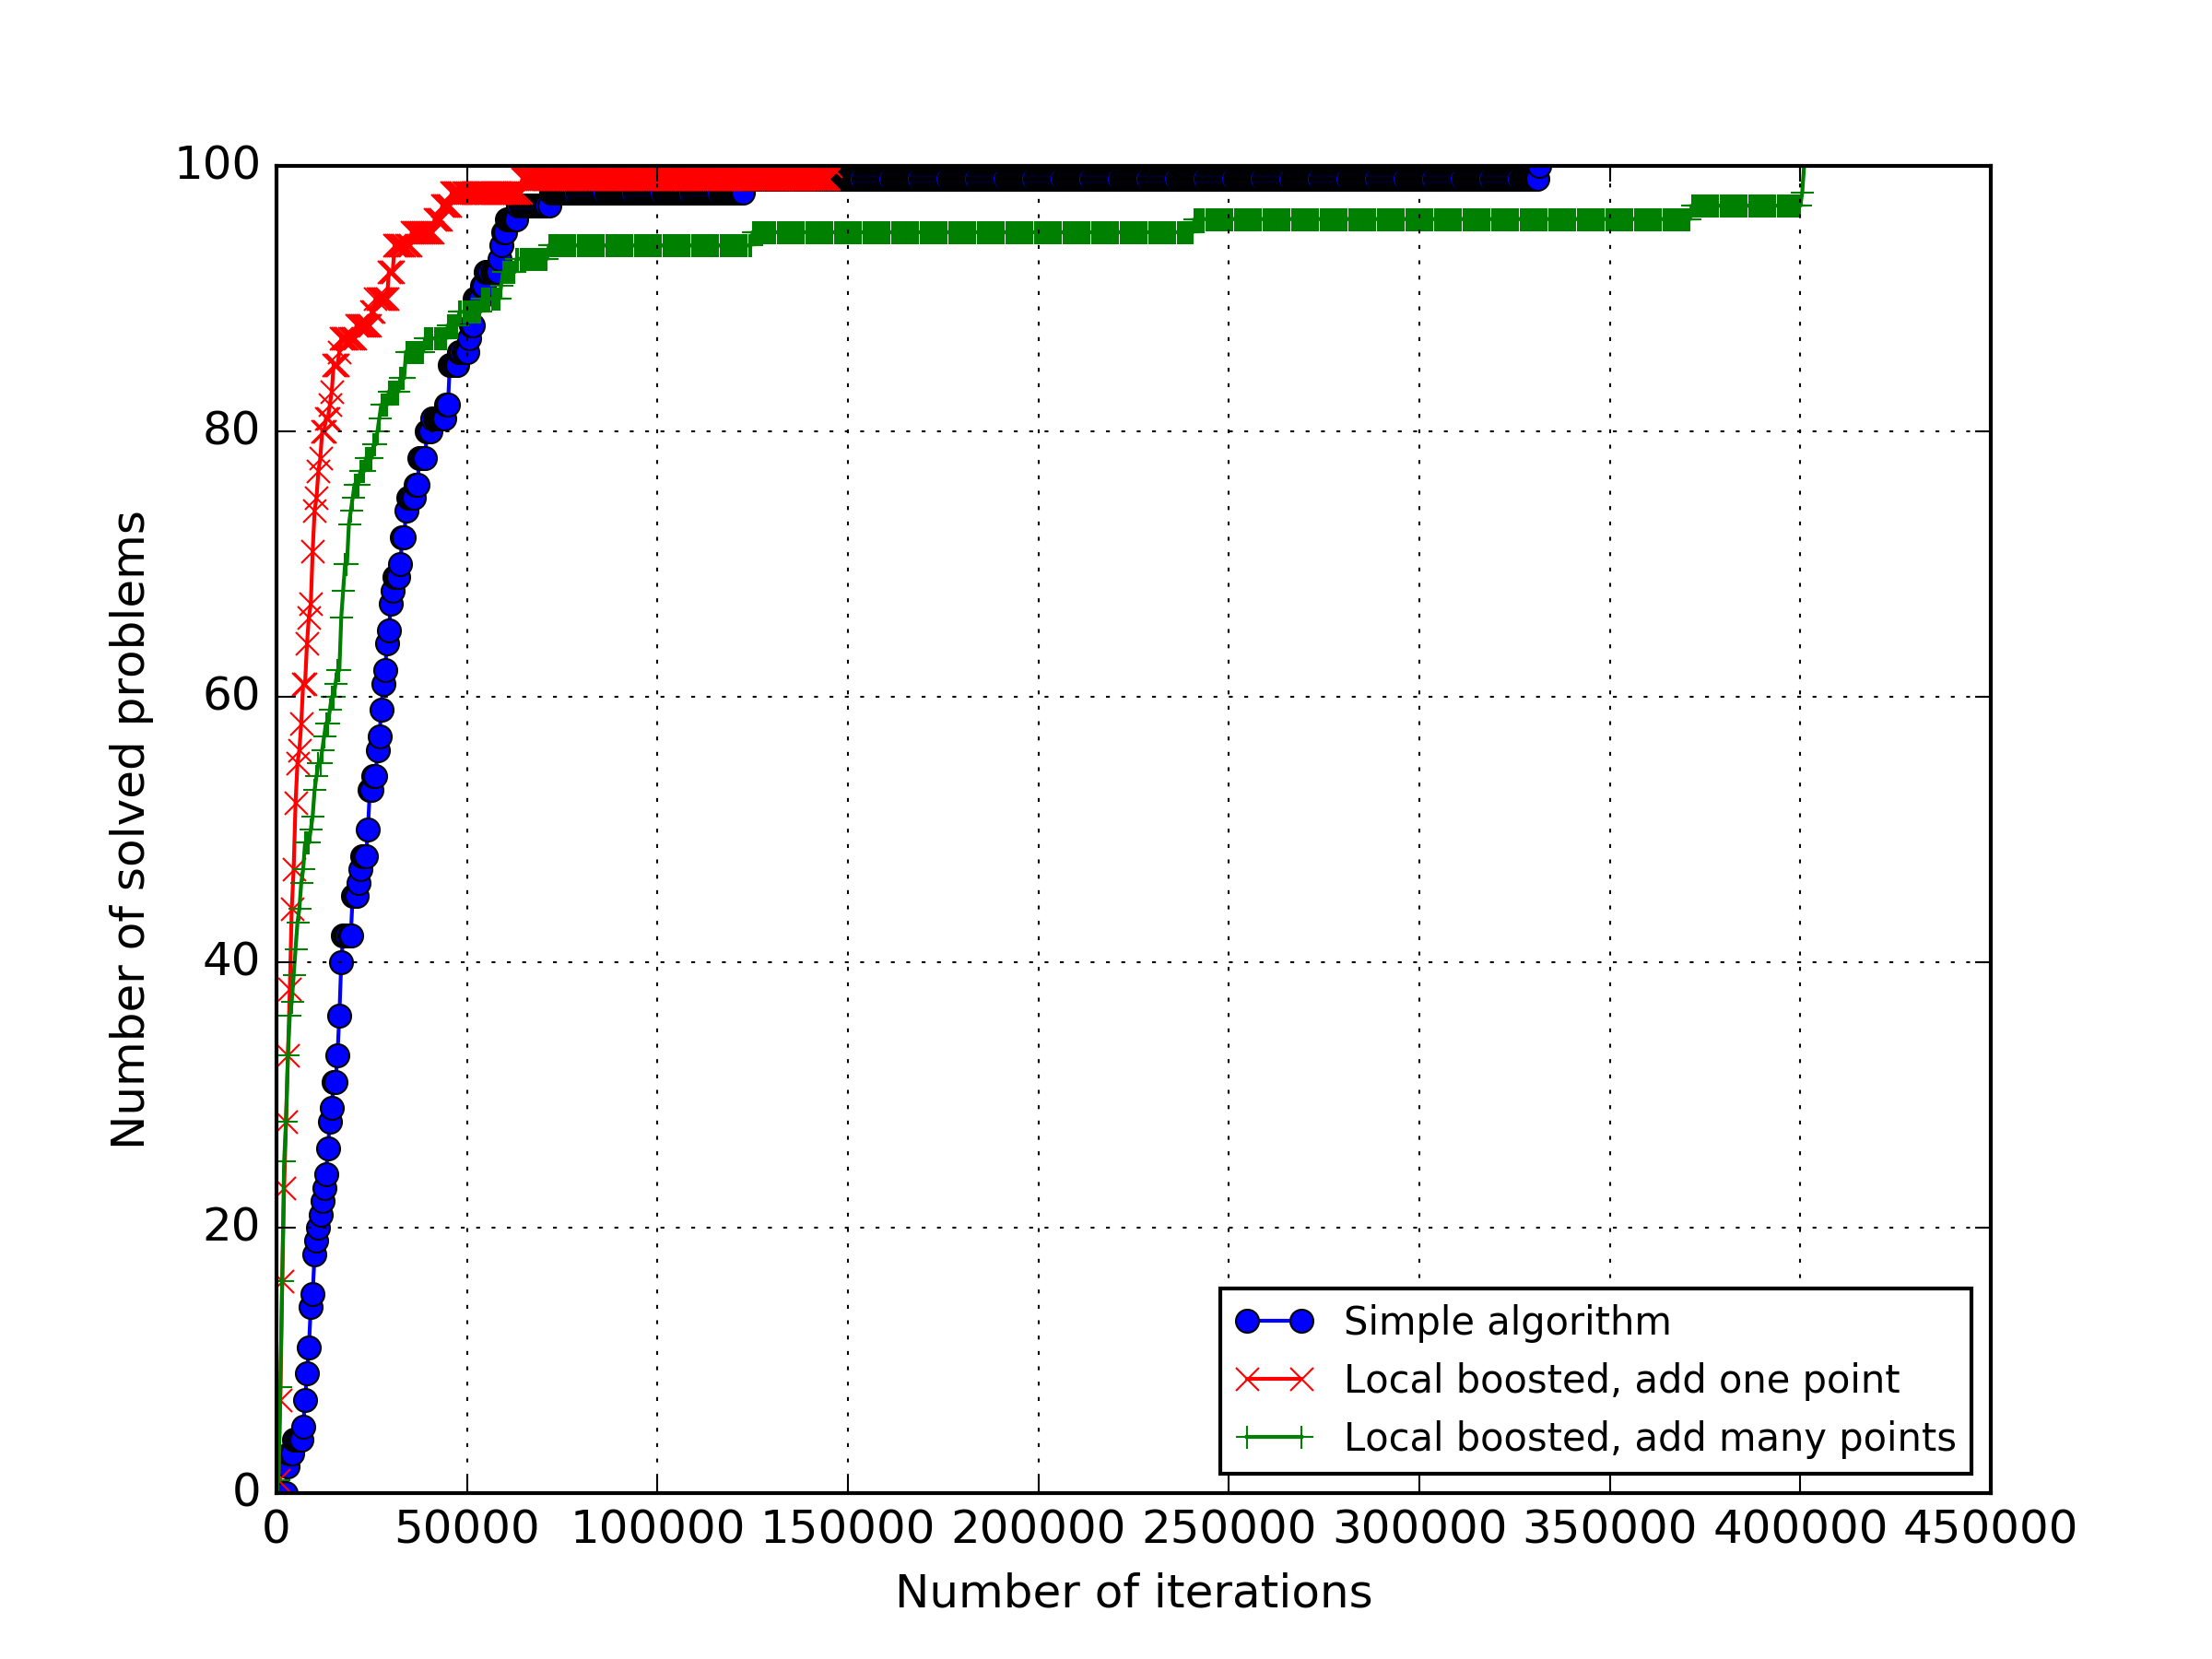
\includegraphics[width=0.75\textwidth]{images/local_search_op.png}
  \caption{Операционные характеристики на классе GKLS 4d Simple при различных вариантах использования локального метода}
  \label{fig:loaclsearchOP}
\end{figure}
Из рис. \ref{fig:loaclsearchOP}, \ref{fig:loaclsearchOP5d} можно сделать вывод, что вариант с использованием только одной лучшей точки, полученной локальным методом, оказался наилучшим.
В обоих случаях он заметно ускорил сходимость глобального алгоритма.
\begin{figure}[ht]
  \center
  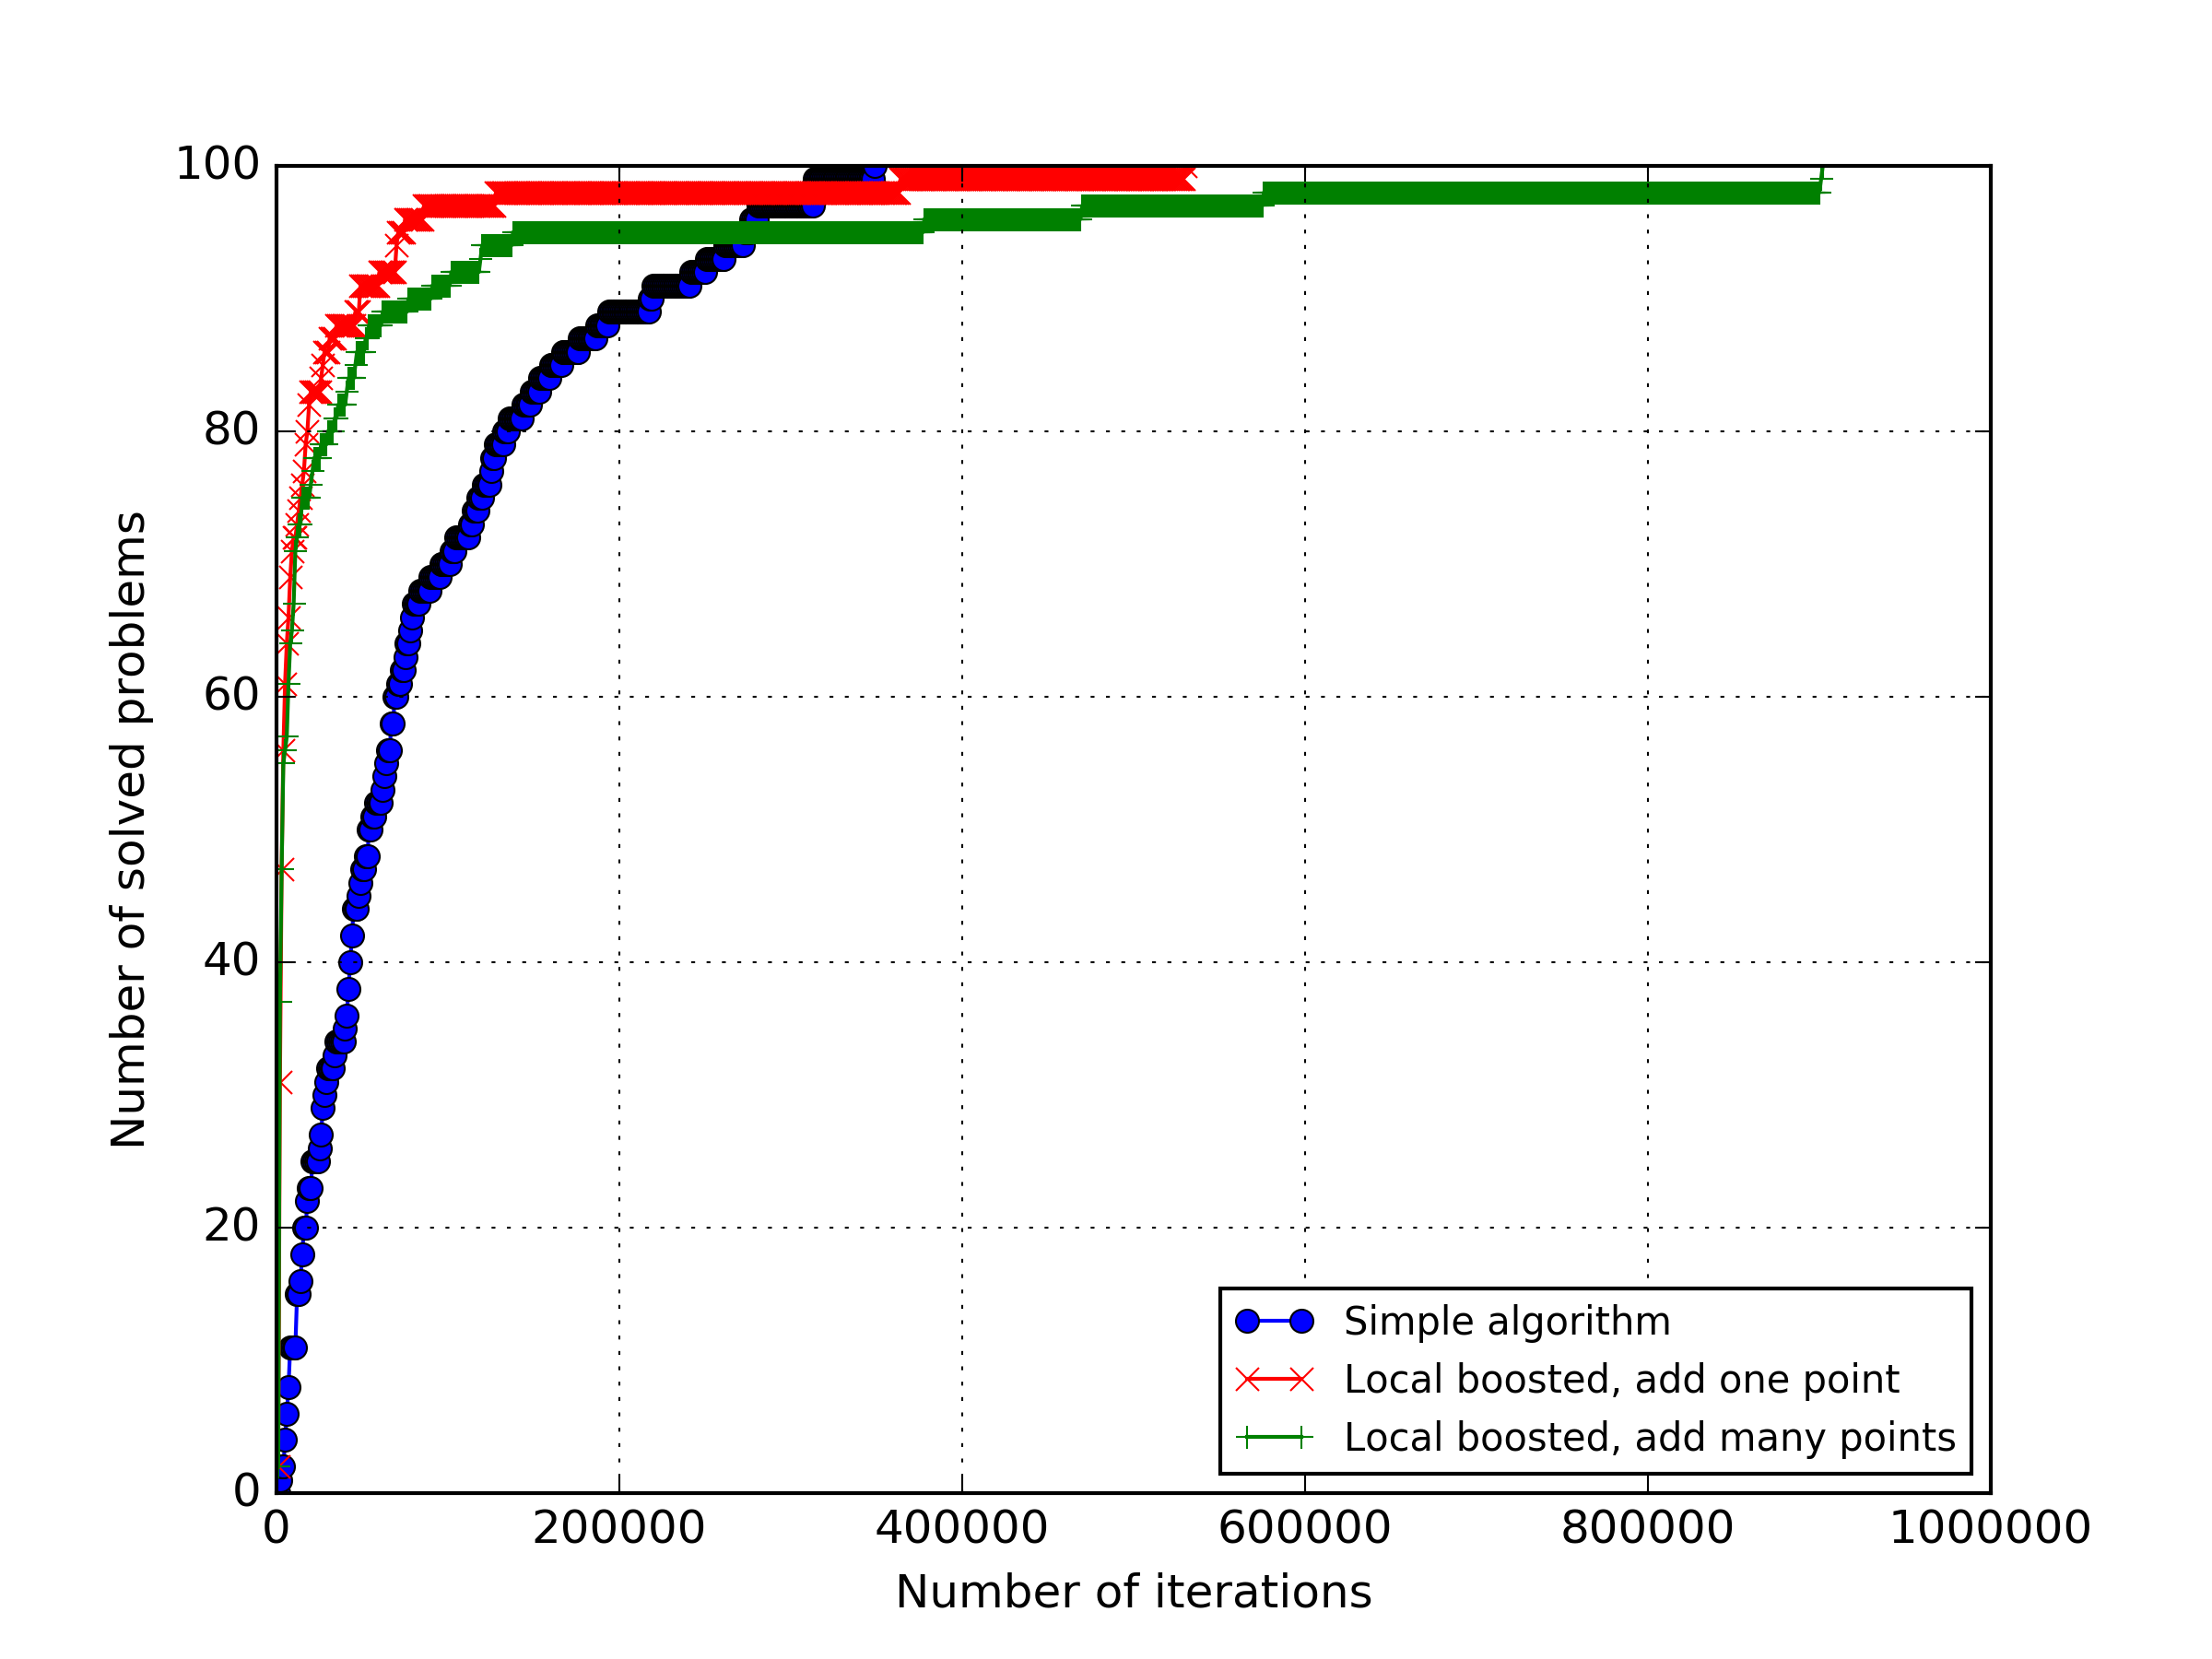
\includegraphics[width=0.75\textwidth]{images/local_search_op5d.png}
  \caption{Операционные характеристики на классе GKLS 5d Simple при различных вариантах использования локального метода}
  \label{fig:loaclsearchOP5d}
\end{figure}

\section{Смешанный алгоритм глобального поиска и его эффективная реализация}
Ещё одной модификацией метода Стронгина, позволяющей при оптимизации лучше учитывать данные о локальных оптимумах, найденных в процессе поиска, является смешанный алгоритм Стронгина-Маркина \cite{mixedAlg}.
Наряду с характеристикой интервала \(R(i)\) (\ref{step3_1}) можно рассматривать \(R^*(i)\), которая будет более чувствиетльна к наличию в интревале текущего найденного минимума функции \(x_k^*\):
\begin{displaymath}
R^*(i)=\frac{R(i)}{\sqrt{(z_i-z^*)(z_{i-1}-z^*)}/\mu + 1.5^{-\alpha}}
\end{displaymath}
где \(f(x_k^*)=z^*\), а \(\alpha \in [1;30]\) --- степень локальности. Чем она больше, тем более высокая характеристика у интервала, содержащего \(x_k^*\), по сравнению с остальными.
\par
Смешанный алгоритм состоит в следующем: в процессе работы метода каждые \(S\) итераций интервал для последующего разбиения выбирается по характеристикам \(R^*(i)\). \(S\) --- параметр смешивания.
Такой подход позволяет существенно ускорить сходимость метода. На рис. \ref{fig:localMixOP4d} приведены операционные характеристики чисто глобального и смешанного алгоритма на классе GKLS 4d Simple.
Параметр смешивания \(S\) равен 5, \(\alpha=15\), остальные параметры метода были заданы такие же, как в разделе \ref{sec:multilev_maps}
\begin{figure}[ht]
  \center
  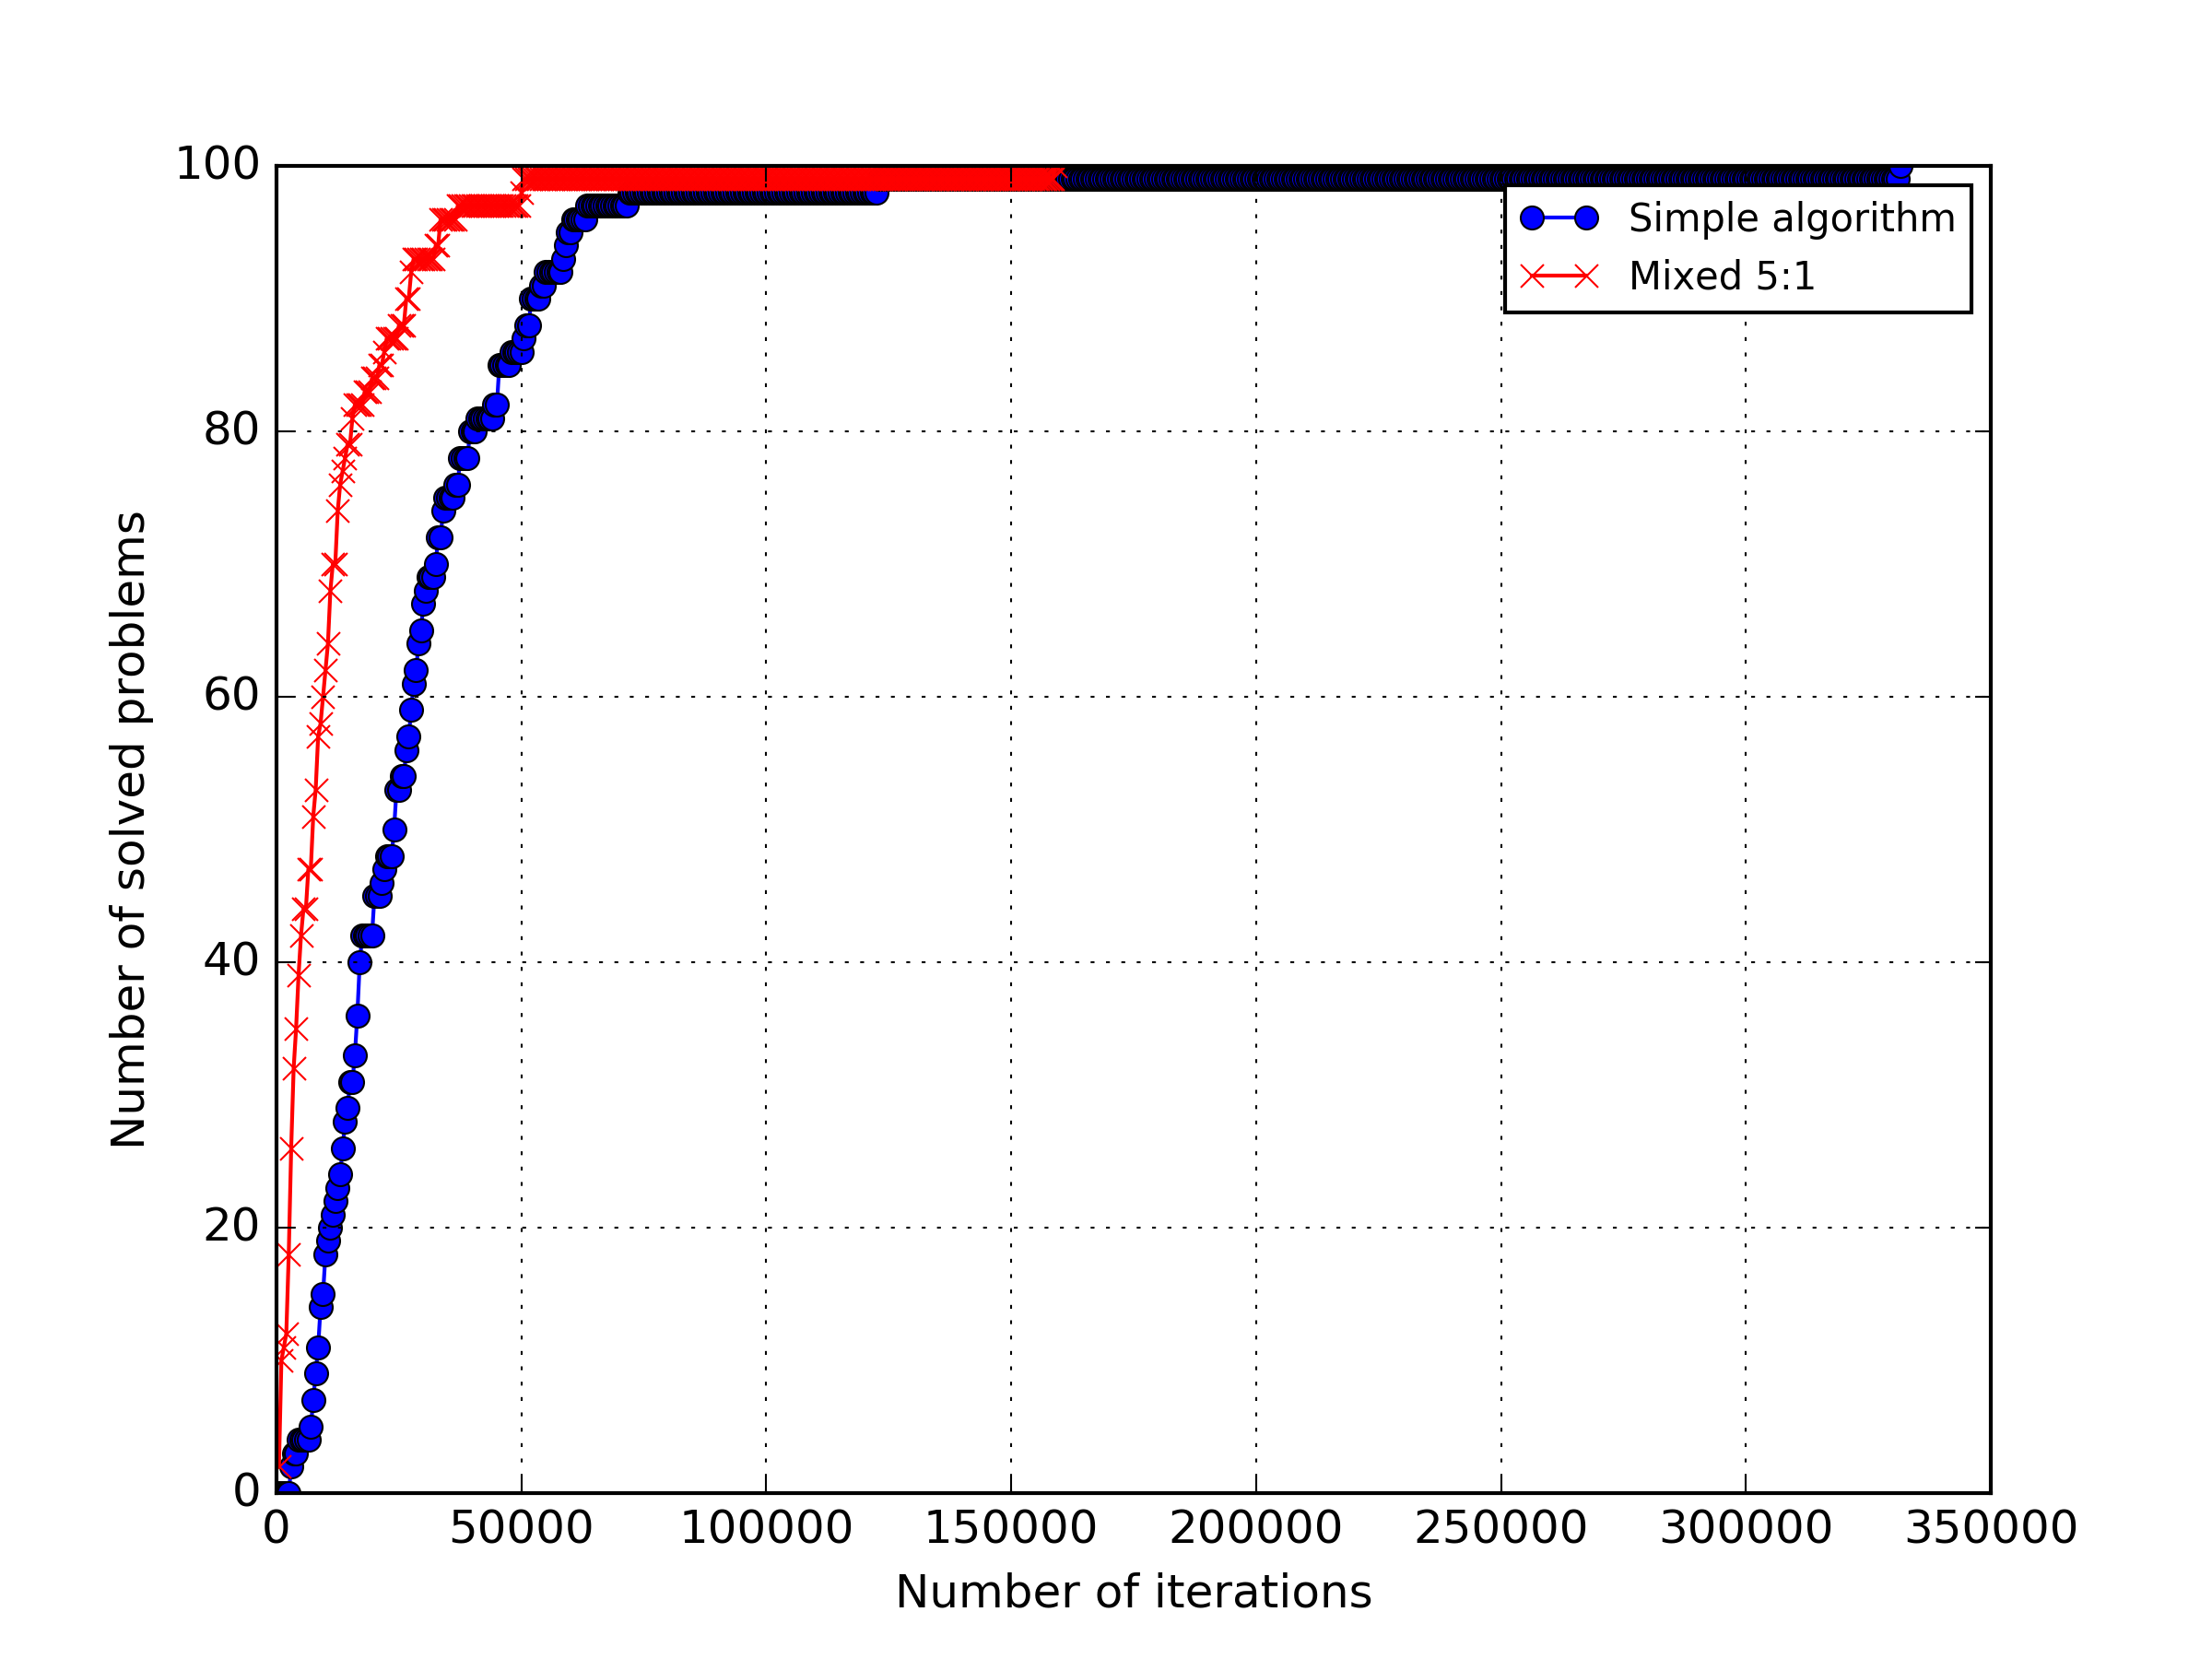
\includegraphics[width=0.75\textwidth]{images/mixed_op4d.png}
  \caption{Операционные характеристики обычного и смешанного АГП на классе GKLS 4d Simple}
  \label{fig:localMixOP4d}
\end{figure}
\par
Из-за того, что интервал имеет сразу две характеристики, появляется проблема эффективной реализации смешанного алгоритма. Если интервал имеет одну характеристику, то для выбора максимальной
достаточно организовать приоритетную очередь характеристик \cite{minmaxheap}.
Причём перезаполнение такой очереди необходимо не на каждой итерации: в большинстве случаев характеристики интервалов не меняются, достаточно удалить разбиваемый интервал и вставить в очередь два новых.
Такая организация работы метода позволяет существенно сократить объём вычислений. При наличии у интервала двух характеристик можно организовать две связанные очереди. В этом случае необходимо предусмотреть
процедуру синхронизации двух очередей.
\par
Перечислим операции, при которых необходима синхронизаия:
\begin{itemize}
  \item вставка интервала сразу в обе очереди;
  \item удаление интервала из какой-либо очереди.
  %\item восстановление внутренней структуры очереди после модификации связанной очереди.
\end{itemize}
\par
Синхронизация достигается путём введения перекрёстных ссылок между элементами очередей. На рис. \ref{fig:heaps} приведена схема связанных очередей. Элемент очереди представляет собой
совокупность ключа (\textbf{LocalR} или \textbf{R}), указателя на интервал (\textbf{pInterval}) и указателя на элемент связанной очереди, соответствующий тому же интервалу (\textbf{pLinkedElement}).
Опишем подробнее алгоритмы вставки и удаления элементов.
\par
Вставка элемента в пару связанных очередей:
\begin{enumerate}
  \item Попытаться вставить элемент в очередь глобальных характеристик (он может быть не вставлен, если имеет слишком низкий приоритет).
  \item Попытаться вставить элемент в очередь локальных характеристик (он может быть не вставлен, если имеет слишком низкий приоритет).
  \item Если элемент интервал вставлен в обе очереди, то выставить перекрёстные ссылки.
\end{enumerate}
\par
Удаление элемента с минимальным ключом:
\begin{enumerate}
  \item Удалить элемент с минимальным ключом из очереди, запомнить указатель \textbf{pLinkedElement}.
  \item Если \textbf{pLinkedElement} ненулевой, то вызвать процедуру удаления элемента, на который указывает \textbf{pLinkedElement} в структуре данных, хранящей связянную очередь.
\end{enumerate}
\par
Последний момент, который надо учесть при реализации: вставка или удаление элемента очереди приводит к тому, что необходимо восстановить её внутреннюю структуру.
Если очередь хранится в куче, то восстанавливается свойство кучеобразности. Во время этого процесса
требуется производить попарные перестановки элементов, а значит, необходимо обновлять ссылки на эти элементы в связанной очереди.
\begin{figure}[ht]
  \center
  \includegraphics[width=0.9\textwidth]{images/examin_heaps.png}
  \caption{Схема устройства связянных очередей}
  \label{fig:heaps}
\end{figure}
\par
Стоит заметить, что внесённые модификации (в основном эта работа со ссылками) не увеличивают ассимптотическую сложность выполнения операций вставки и удаления по сравнению с единственной очередью.

\section{Многоуровневая схема редукции размерности с помощью разверток}
\label{sec:multilev_maps}
Теоретически с помощью развёрток можно решить задучю любой размерности, однако на ЭВМ развёртка строится с помощью конечноразрядной арифметики, из-за чего, начиная с некоторого \(N^*\),
построение разветки невозможно (значение \(N^*\) зависит от максимального количества значащих разрядов в арифметике с плавающей точкой).
Понять почему это происходит нетрудно, обратившись, например к \cite{strOptBook}.
\par
Чтобы преодолеть эту проблему профессором В. П. Гергелем была предложена следующая идея: использовать композицию развёрток меньшей размерности для построения отображения
\(z(x): [0;1] \rightarrow D \in \mathbf{R}^N\).
Поясним эту схему на примере редукции размерности в четырёхмерной задаче. Пусть \(y_2(x)\) --- двухмерная развёртка (отображает отрезок в прямоугольник), тогда рассмотрим функцию
\(\psi(x_1,x_2)=\varphi(y_2(x_1), y_2(x_2))\). К \(\psi(x_1,x_2)\) можно также применить редукцию размерности с помощью развёртки. Таким образом, задав точку \(x^*\in [0;1]\),
вычислив \(y_2(x^*)=(x_1,x_2)\) и пару векторов \((y_2(x_1), y_2(x_2))\), получим четырёхмерную точку. Из инъективности \(y_2(x)\) следует инъективность \(z(x)\).
\par
Проблемой этого подхода является выяснение свойств функции \(\varphi(z(x))\) и возможности использования одномерного метода Стронгина с гёльдеровой метрикой для оптимизации \(\varphi(z(x))\).
Чтобы не тратить время на теоретическое исследование, были проведены численные эксперименты с целью оценить возможность применения многоуровневой развёртки в четырёхмерном случае.
\par
Прежде всего, рассмотрим линии уровня функции \(\psi(x_1,x_2)=\varphi(y_2(x_1), y_2(x_2))\) при \(\varphi(t)=\sum_{i=1}^{4}(t_i-0.5)^2\).
\begin{figure}[ht]
  \center
  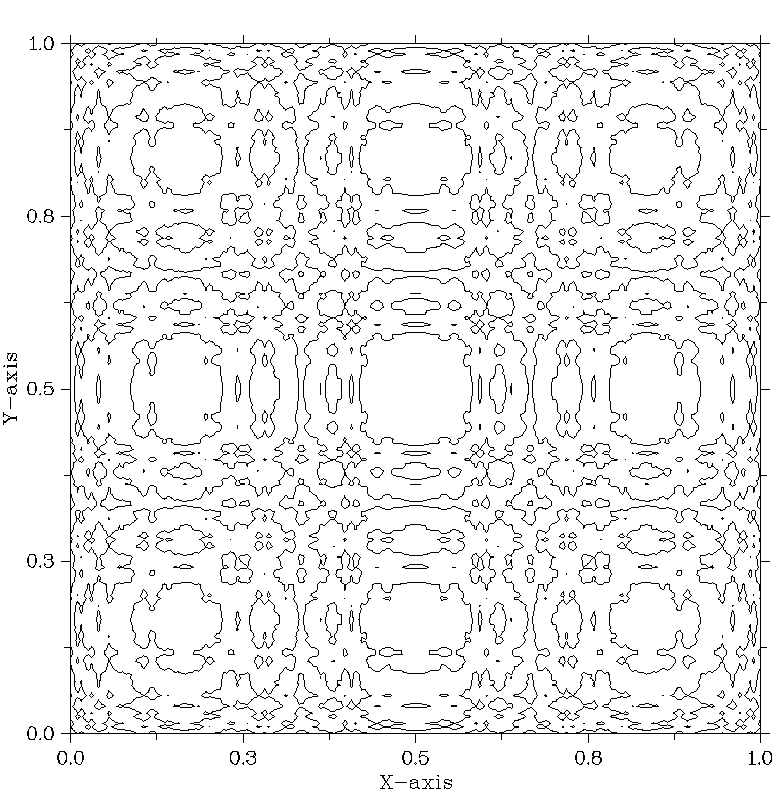
\includegraphics[width=0.55\textwidth]{images/multimap_isolines.png}
  \caption{Линии уровня функции \(\psi(x_1,x_2)=\varphi(y_2(x_1), y_2(x_2))\)}
  \label{fig:1}
\end{figure}
Как видно из рис. \ref{fig:1}, линии уровня имеют довольно сложную структуру, что говорит о возможных сложностях применения одномерного метода с разверткой.
\par
Далее был проведён более масштабный вычислительный экспеимент: с помощью многоуровневой развертки решались 100 задач из класса GKLS 4d Simple. На рис. \ref{fig:multimapOP} приведены операционные
характеристики метода с простой и многоуровневой развёртками. При этом были зафиксированы следующие параметры алгоритма: надёжность \(r=4.5\), плотность построения всех развёрток 12, критерий остановки попадание
точки, поставленной методом в квадрат со стороной \(\varepsilon=10^{-2}\), центром которого является решение задачи.
\begin{figure}[ht]
  \center
  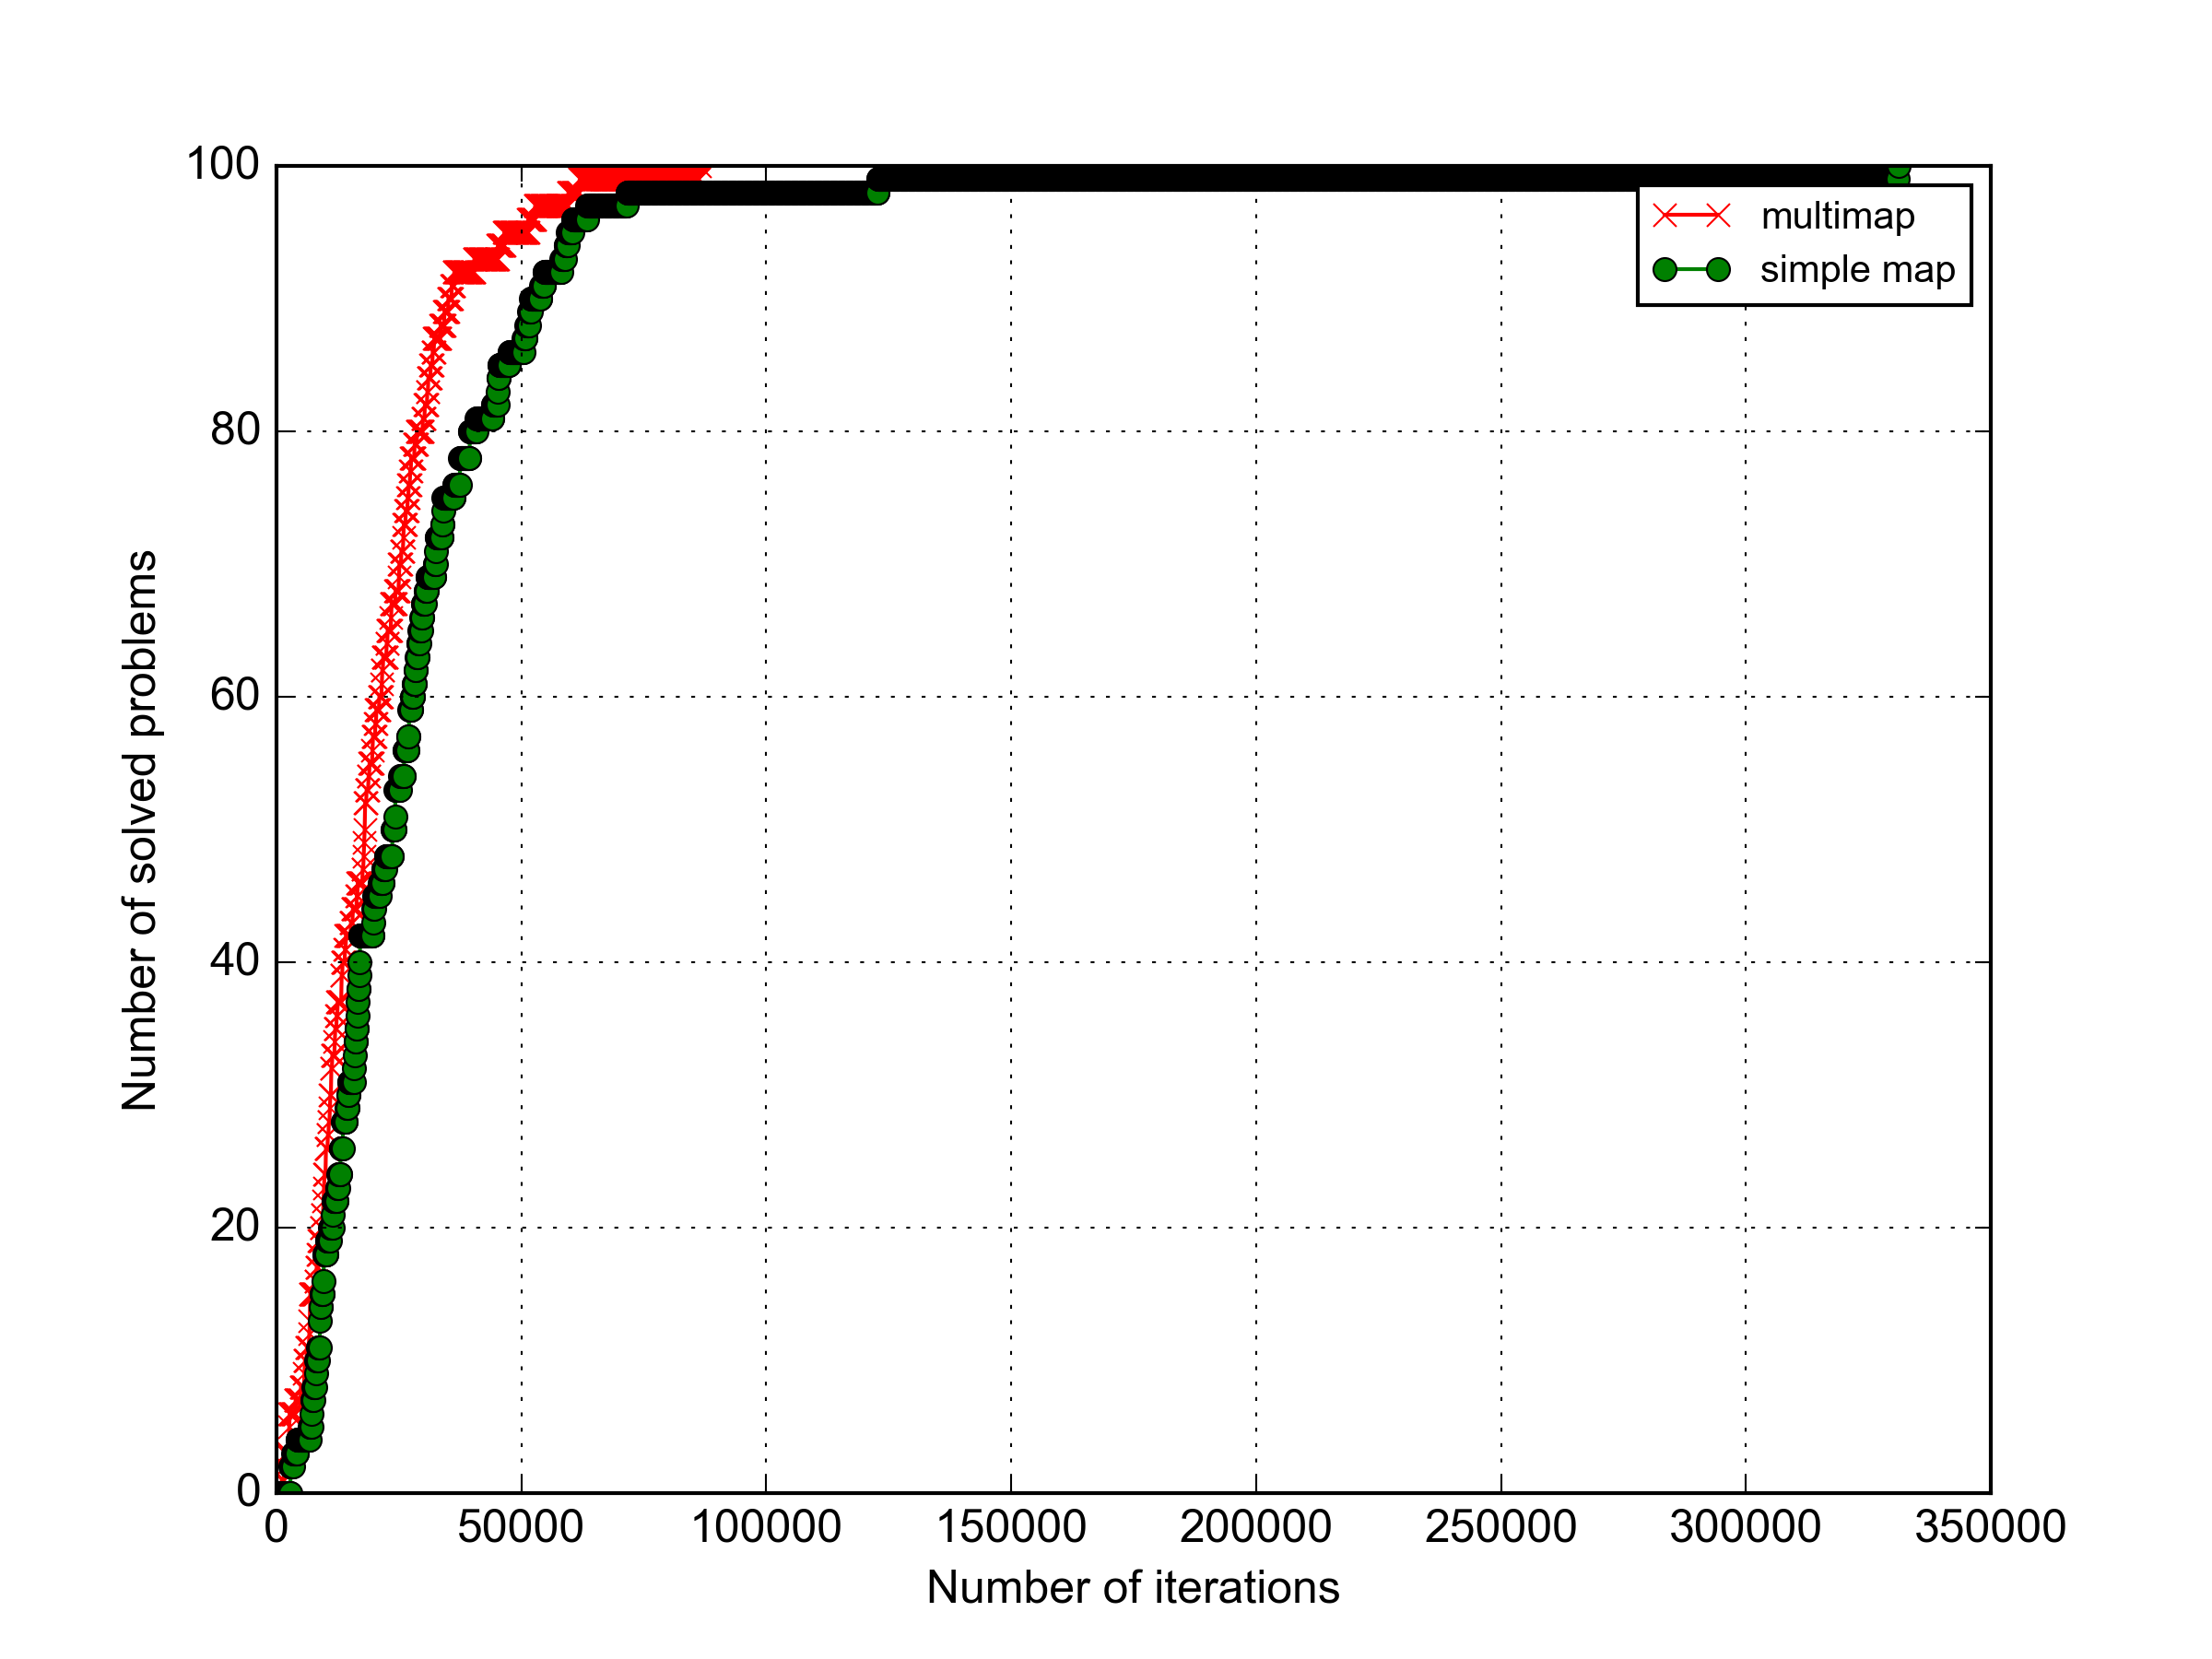
\includegraphics[width=0.75\textwidth]{images/multimap_op.png}
  \caption{Операционная характеристика метода с различными развёртками на классе GKLS 4d Simple}
  \label{fig:multimapOP}
\end{figure}
Как видно из графика, операционная характеристика метода с многоуровневой развёрткой лежит выше, чем аналогичная кривая метода с простой развёрткой. Кроме того, метод с многоуровневой развёрткой
заметно раньше вышел на стопроцентную надёжность на решаемой выборке задач. Исходя из первых экспериментов можно сказать, что при данных параметрах алгоритма многоуровневая развертка лучше, но
при уменьшении точности алгоритма \(\varepsilon\) до значения \(10^{-3}\) выполнения критерия остановки в случае использования многоуровневой развёртки с выбранной плотностью построения внутренних развёрток не происходит.
Если плотность увеличить до 16, то остановка также не будет происходить. Исходя из этого можно делать вывод, что использование на практике многоуровневых развёрток с большой долей вероятности
невозможно из-за описанного дефекта сходимости.

\section{Применение локальных оценок константы Гёльдера для ускорения сходимости АГП}
В части работы будем рассматривать задачу глобальной оптимизации в постановке без функциональных ограничений.
Как видно из описания метода, независимо от локальных свойств оптимизируемой одномерной
функции, для вычисления характеристик всех интервалов (\ref{step3_1}) используется одно и то же
значение оценки константы Гёльдера (\ref{step2}). В работе \cite{sergLocalTuningFirst} было предложено использовать различные
значения \(M=\mu_1\), (\(\mu_1\) из (\ref{step2}) при \(\nu=1\)) в случае отсутствия функциональных ограничений), (\ref{step3_1})) для каждого интревала, а
также показана эффективность такого подхода в случае одномерной оптимизации функций,
удовлетворяющих условию Липшица. В работе \cite{nestedLocal} рассмотрено применение
адаптивных оценок констант Липшица в схеме многомерной вложенной оптимизации.

Для каждого интревала локальная оценка константы является максимум-аддитивной свёрткой
<<глобальной>> и <<локальной>> компонент (\(\gamma\) и \(\lambda\) соответственно):
\begin{displaymath}
  \begin{array}{lr}
    \lambda_i=\max\{H_{i-1},H_i,H_{i+1}\} \\
    H_i=\frac{|z_i-z_{i-1}|}{\Delta_i} \\
    H^k=\max\{H_i:i=2,\dots ,k\} \\
    \gamma_i=H^k\frac{\Delta_i}{\Delta^{max}} \\
    \Delta^{max}=\max\{\Delta_{i}:i=2,\dots ,k\}
  \end{array}
\end{displaymath}
\begin{equation}
\label{additiveConv}
M_i=r\cdot \max\{H_i, \frac{1}{2}(\lambda_i+\gamma_i),\xi\}
\end{equation}

Параметр \(\xi\) предотвращает обнуление оценки \(M_i\) в случае, если оптимизируемая
фнкция является тождественной константой, и выбирается достаточно малым.
Данный вариант свёртки не зависит от параметра \(r\), однако в \cite{sergLocalTuning}
также рассматриваетсяи адаптивная свёртка:
\begin{equation}
\label{additiveAdaptiveConv}
M_i=r\cdot \max\{H_i, \frac{\lambda_i}{r}+\frac{r-1}{r}\gamma_i,\xi\}
\end{equation}

Если априори известно, что оптимизируемая функция имеет сложный рельеф с множеством
локальных минимумов, то \(r\) изначально задаётся большим, что ведёт к преобладанию в
адаптивной свёртке «глобальной» сооставляющей \(\gamma\).

Оба варианта свёртки (\ref{additiveConv}), (\ref{additiveAdaptiveConv}) были предложены
и детально рассмотрены в \cite{sergLocalTuning} для случая одномерных функций,
удовлетворяющих условию Липшица. В данном разделе будет рассмотрено применение этих
свёрток для оптимизации двумерных функций в случае редукции размерности с помощью развёрток.

В \cite{sergLocalTuning} приведена теорема о сходимости метода в случае, если целевая функция
липшицева, однако, как правило, подобные утверждения справедливы и в Гёльдеровой метрике, поэтому,
предположительно, будет верна следующая гепотеза:
\begin{hypothesis}
Пусть целевая функция \(f(x)\) удовлетвворяет условию Гёльдера с конечной константой
\(H > 0\), и пусть \(x\) является предельной точкой последовательности \(\{x_k\}\),
порождаемой алгоритмом. Тогда верны следующие утверждения:
\begin{enumerate}
  \item Если \(x\in(0;1)\), то сходимость к точке \(x\) является двухсторонней, т.е.
  существуют две подпоследовательности \(\{x_k\}\), сходящиеся к \(x\): одна слева,
  а другая справа;
  \item \(f(x_k) \geqslant f(x)\) для всех точек испытаний \(x_k, k \geqslant 1\);
  \item Если существует другая предельна точка \(x^* = x\), то \(f(x) = f(x^*)\);
  \item Если функция \(f(x)\) имеет конечное число локальных минимумов на отрезке \([0, 1]\),
  то точка \(x\) является локально оптимальной;
  \item (Существенное условие сходимости к глобальномк минимуму). Пусть \(x^*\)
  является глобальным минимумом \(f(x)\). Если существует такое число \(k^*\),
  что для всех итераций с номерами \(k > k^*\) неравенство
  \(M_j(k) > H_j(k)\) выполняется, где \(H_j(k)\) --- это константа Гёльдера на интервале
  \([x_{j(k)-1}, x_{j(k)}]\), содержащем \(x^*\), а \(M_{j(k)}\) её оценка.
  Тогда множество предельных точек последовательности \(\{x_k\}\) совпадает с множеством
  глобальных минимумов функции \(f(x)\).
\end{enumerate}
\end{hypothesis}

Доказательство гепотезы требует отдельных теоретических исследований. В рамках данной
работы оно не будет проведено, наличие сходимости установлено только численно.

Эксперименты по оценке эффективности метода с локально-адаптивной оценкой константы
Гёльдера производились на двумерных классах задач Гришагина (\(F_{GR}\))
и GKLS Simple 2d, упомянутых в разделе \ref{subsec:test_problems}
Каждый из классов содержит 100 многоэкстремальных функций. Развёртка во всех экспериментах
строилась с плотностью \(m=12\), параметр \(\varepsilon\) в критерии остановки был равен \(10^{-3}\).
Параметр \(r\) выбирался минимально возможным, при котором заданный метод решает все
задачи класса. Шаг поиска \(r\) равен \(0.1\).

\begin{figure}[ht]
    \centering
    \subfloat[глобальная оценка \(H\)]{{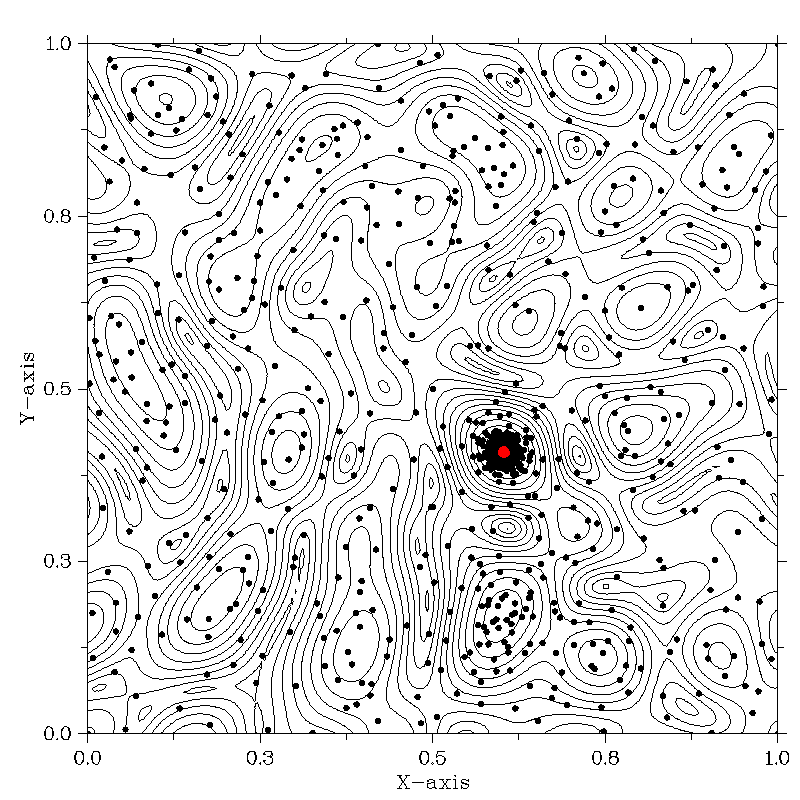
\includegraphics[width=0.45\textwidth]{images/gs_glob.png} }}
    \qquad
    \subfloat[локально-адаптивная оценка \(H\)]{{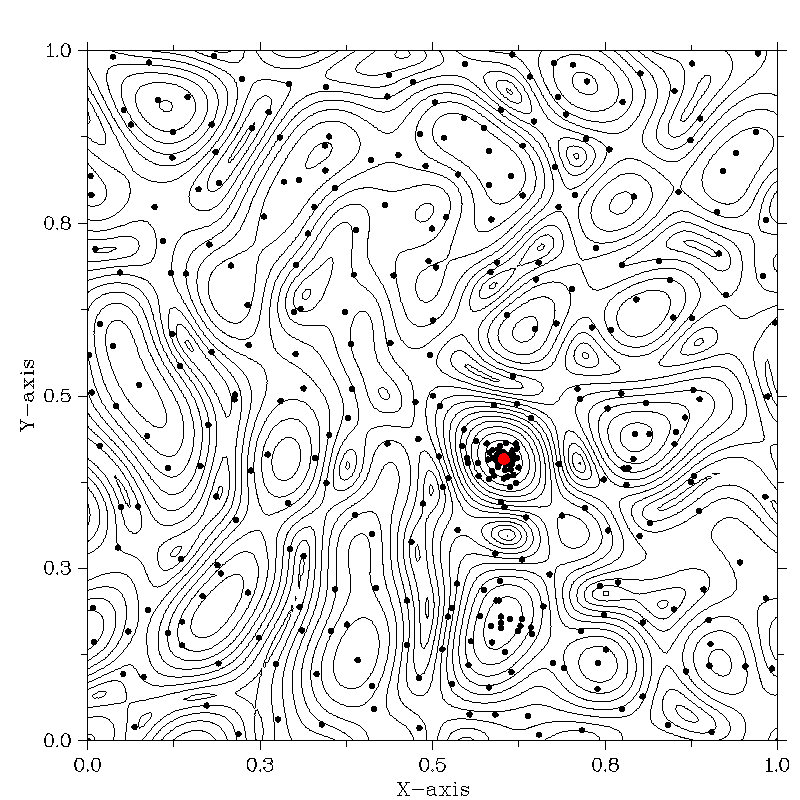
\includegraphics[width=0.45\textwidth]{images/gs_loc.png} }}
    \caption{Линии уровня одной из функций класса \(F_{GR}\)}
    \label{fig:grish_isolines}
\end{figure}

Для наглядной иллюстрации преимущества локально-адаптивной схемы оценки константы
\(H\) рассмотрим результаты работы метода на конкретном примере. На рис. \ref{fig:grish_isolines} показаны
линии уровня одной из функций класса \(F_{GR}\) и точки испытаний, проведённых методом с глобальной
оценкой константы Гёльдера и с оценкой по формуле (\ref{additiveConv}). Как видно из рисунков, метод с
глобальной оценкой константы проводит большое число испытаний в окрестности точки
глобального минимума прежде (всего проведено 1086 испытаний), чем выполнится условие
остановки, в то врямя, как метод с локально-адаптивной оценкой гораздо быстрее
сходится (всего проведено 385 испытаний). Аналогичная ситуация имеет место при
оптимизации одной из функций класса GKLS Simple 2d (рис. \ref{fig:gkls_isolines}). Метод с глобальной
оценкой константы произвёл 2600 испытаний, а метод с локально-адаптивной оценкой – 1190.

\begin{figure}[ht]
    \centering
    \subfloat[глобальная оценка \(H\)]{{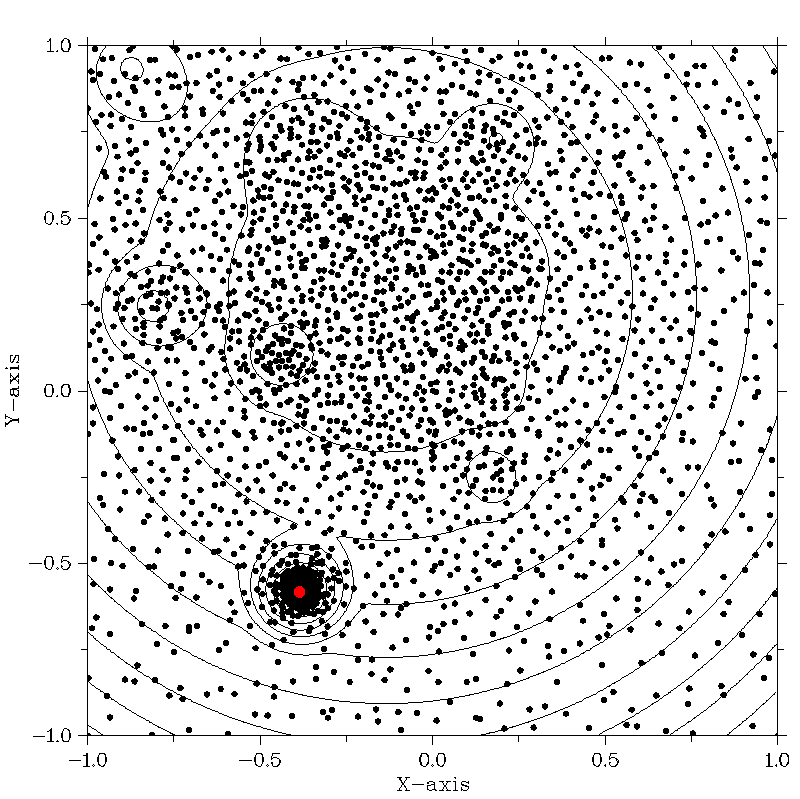
\includegraphics[width=0.45\textwidth]{images/gkls_glob.png} }}
    \qquad
    \subfloat[локально-адаптивная оценка \(H\)]{{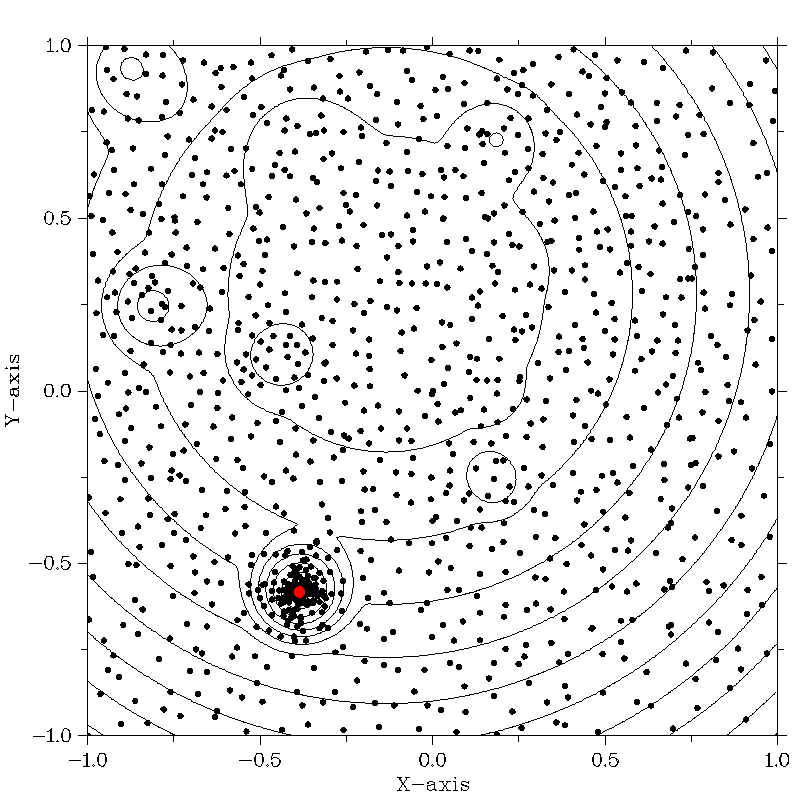
\includegraphics[width=0.45\textwidth]{images/gkls_loc.png} }}
    \caption{Линии уровня одной из функций класса GKLS Simple 2d}
    \label{fig:gkls_isolines}
\end{figure}

\begin{figure}[ht]
    \center
    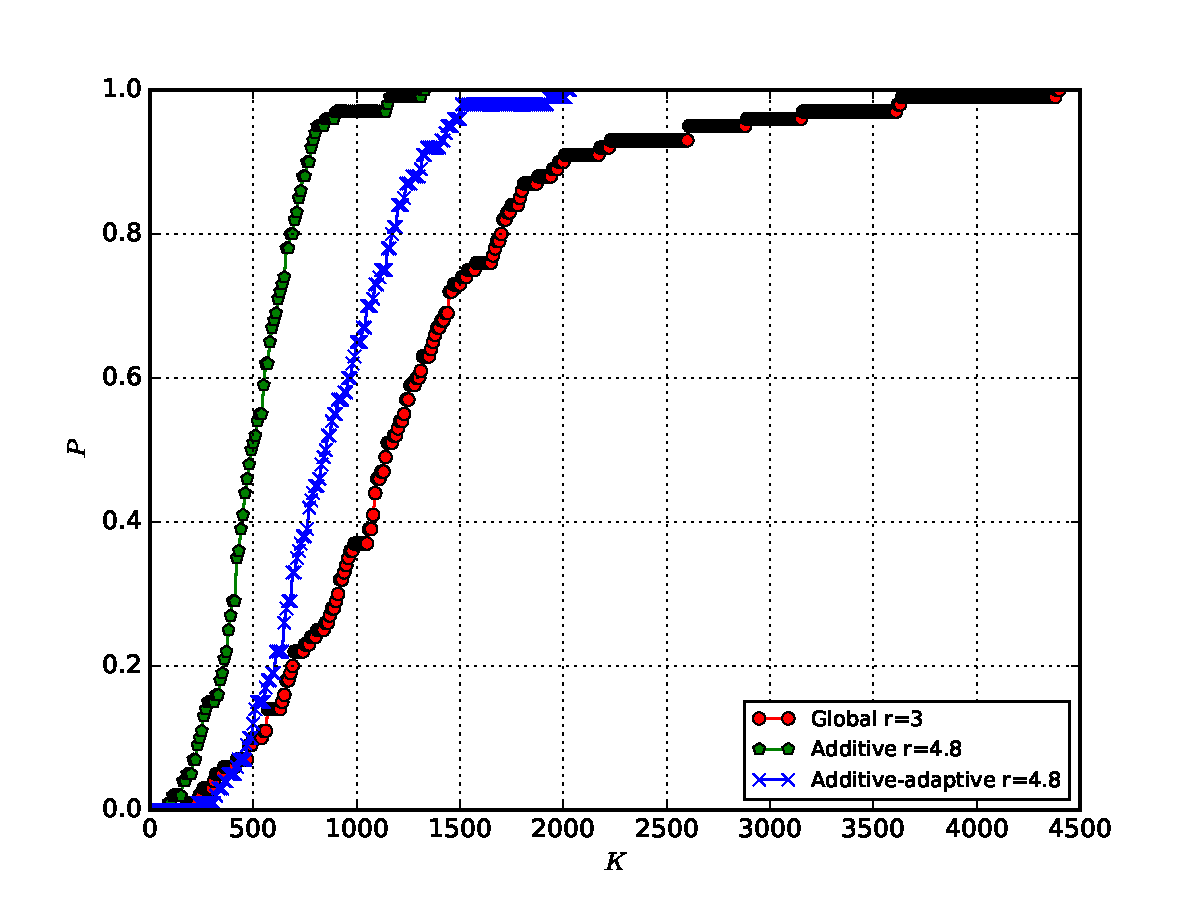
\includegraphics[width=0.75\textwidth]{images/grishagin.pdf}
    \caption{Операционные характеристики методов на классе задач \(F_{GR}\)}
    \label{fig:grishh_op}
\end{figure}

\begin{figure}[H]
  \center
  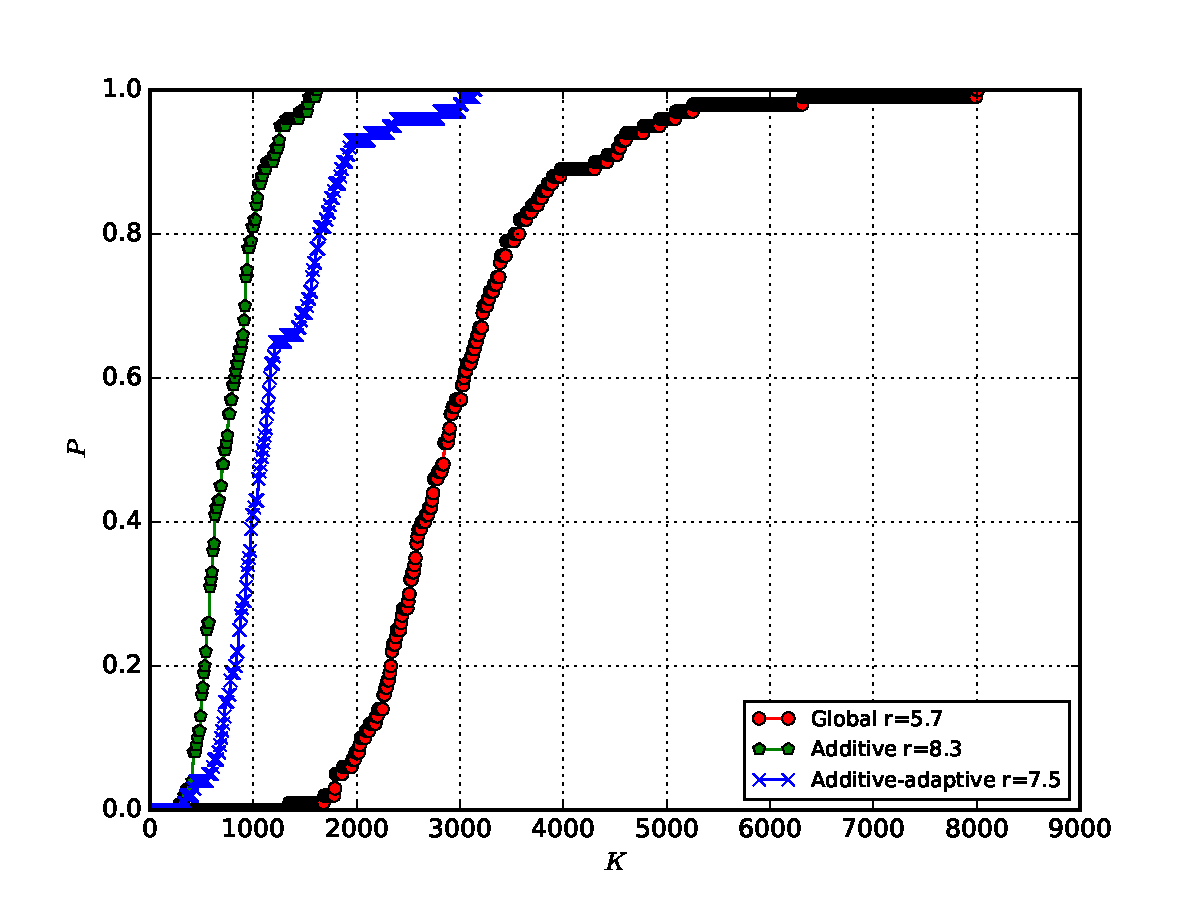
\includegraphics[width=0.75\textwidth]{images/gkls-s.pdf}
  \caption{Операционные характеристики методов на классе задач GKLS Simple 2d}
  \label{fig:gkls_op}
\end{figure}

Далее перейдём к сравнению различных вариантов метода на рассматриваемых классах задач.
В качестве оценки эффективности алгоритма будем использовать, операционную характеристику,
описанную в разделе \ref{subsec:methods_compasion}

Как видно из операционных характеристик на рис. \ref{fig:grishh_op} и \ref{fig:gkls_op},
оба метода с локально-адаптивной оценкой константы Гёльдера показали существенное преимущество, однако они требуют
задавать более высокое значение параметра \(r\). Если сравнивать между собой методы с
адаптивной и неадаптивной свёрткой (\ref{additiveConv}), (\ref{additiveAdaptiveConv}), то наглядно видно преимущество последнего,
хотя он и требует большее значение параметра надёжности \(r\) для решения задач из класса GKLS.

\section{Прикладная задача поиска оптимального управления}
\label{sec:optimal_cpntrol}
Задача глобальной оптимизации возникает при синтезе оптимальных с точки зрения некоторых
критериев управлений в линейных системах ОДУ. Если управление является линейной обратной
связью по состоянию, то система с управлением имеет вид:
\begin{equation}
  \label{eq:control_system}
    \dot x = (A+B_u\Theta)x + B_v v, x(0)=0,
\end{equation}
где  \(v(t)\in L_2\) --- некоторое возмущение.
Выходы системы описываются формулами \(z_k=(C_k+B_u\Theta),k=\overline{1,N}\).
Вляиние возмущения на \(k\)-й выход системы описывается критерием
\begin{displaymath}
  J_k(\Theta)=\sup_{v\in L_2} \frac{\max_{1\le i \le n_k} \sup_{t\ge 0}|z_k^{(i)}(\Theta,t)|}{||v||_2}.
\end{displaymath}

Нужно найти компоненты вектора \(\Theta\), минимизирующие один из критериев при
заданных ограничениях на другие:
\begin{displaymath}
   J_1(\Theta^*)=\min\{J_1(\Theta):J_k(\Theta)\leqslant S_k,k=\overline{2,N}\}.
\end{displaymath}

В \cite{optControl} указан способ вычисления критериев, состоящий в следующем:
\begin{itemize}
\item найти матрицу \(Y\) из уравнения:
\begin{displaymath}
  (A+B_u\Theta)Y+Y(A+B_u\Theta)^\mathsf{T}+B_v B_v^\mathsf{T} = 0
\end{displaymath}
\item если \(Y\) положительно определена, то используя её, вычислить функционалы \(J_k(\Theta)\):
\begin{displaymath}
  J_k(\Theta)=\sqrt{\max_{1\leqslant i\leqslant n_k}\{(C_k^{(i)}+D_k^{(i)}\Theta)Y(C_k^{(i)}+D_k^{(i)}\Theta)^\mathsf{T}\}},k=\overline{1,N},
\end{displaymath}
где \(C_k^{(i)},D_k^{(i)}\) --- \(i\)-е строки матриц \(C_k\) и \(D_k\) соответственно.
\end{itemize}

Для предотвращения случаев, когда \(Y\) незнакоопределена, в качестве дополнительного ограничения
использовался критеий устойчивости линейной системы ОДУ: все действительные части
собственных чисел матрицы \(A+B_u\Theta\) должны быть отрицательны:
\begin{displaymath}
  g_0(\Theta)=\min_{j}\re(\lambda_j(\Theta)) < 0
\end{displaymath}

С целью проверки корректности реализации вычисления критериев задачи
индексным алгоритмом глобального поиска были решены две задачи рассматриваемого типа
(их решение также приведено и в \cite{optControl}).

В задаче виброзащиты параметры системы (\ref{eq:control_system}) определются следующим
образом:
$$
A=\begin{bmatrix}
    0       & 1 \\
    0       & 0 \\
\end{bmatrix},
B_v=B_u=\begin{bmatrix}
  0       \\
  1       \\
\end{bmatrix},
C_1=\begin{bmatrix}
  0     & 1
\end{bmatrix},D_1=0,
C_2=\begin{bmatrix}
  0     & 1
\end{bmatrix},D_2=1.
$$

Управление имеет вид \(u=[\theta_1,\theta_2]x\), где \(\theta_1 \leqslant 0,\theta_2\leqslant 0\) ---
оптимизируемые параметры. Сама задача ставится следующим образом:
\begin{equation}
  \label{eq:opt_ctrl_problem}
  J_2(\Theta^*)=\min\{J_2(\Theta):J_1(\Theta)\leqslant 1, g_0(\Theta)\leqslant -0.02\}.
\end{equation}

\begin{figure}[ht]
  \center
  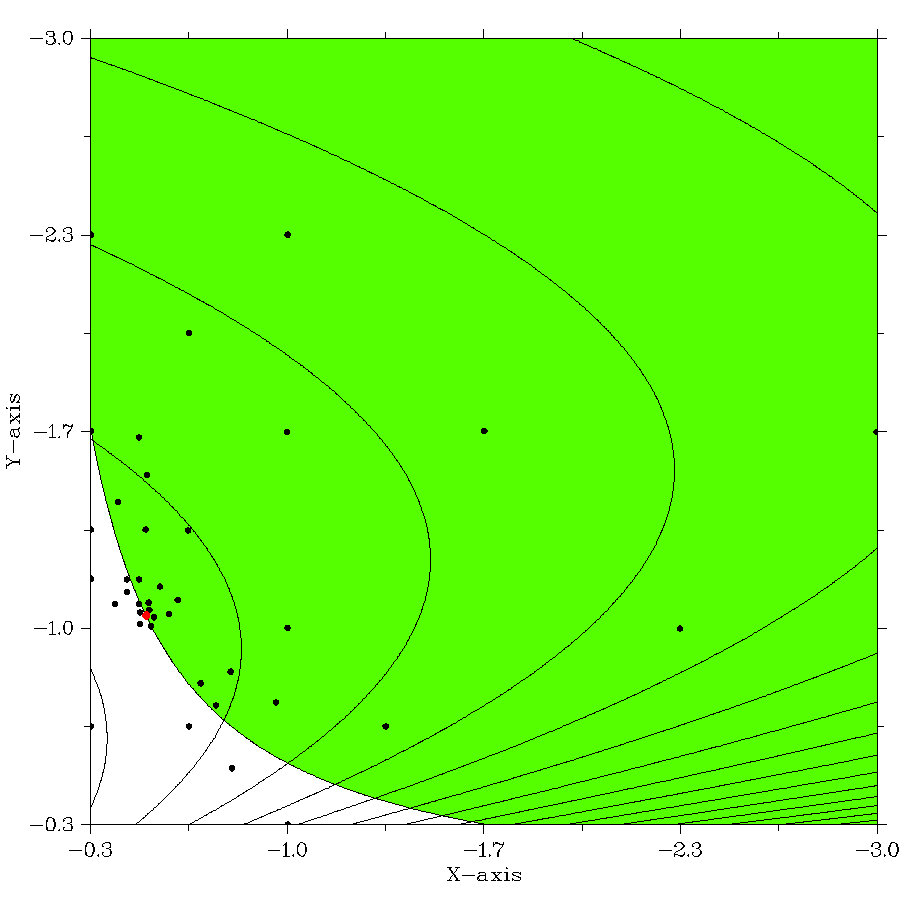
\includegraphics[width=0.55\textwidth]{images/controlProblem.png}
  \caption{Линии уровня для задачи виброзащиты с отмеченными точками испытаний АГП}
  \label{fig:controlProblem}
\end{figure}
При решении этой задачи АГП с параметрами \(r=2.3\), \(\varepsilon=10^{-2}\) произвёл
65 испытаний, причём целевая функция была вычислена 27 раз. Найдена оптимальная точка с координатами
\(\widetilde\theta_1 =-0.503223,\widetilde\theta_2=-0.997168\), \(J_2(\widetilde\Theta)=0.866551\),
а ограничение на \(J_1\) активно.
На рис. \ref{fig:controlProblem}
представлены линии уровня целевой функции задачи виброзащиты. В данном случае допустимая область (закрашена на рисунке)
имеет довольно простую границу, а целевая функция унимодальна.

В задаче гашения колебаний параметры системы (\ref{eq:control_system}) определются следующим
образом:
$$
A=\begin{bmatrix}
  0  & 0 & 1 & 0 \\
  0  & 0 & 0 & 1 \\
  -2  & 1 & -2\beta & \beta \\
  1  & -1 & \beta & -\beta \\
\end{bmatrix}, \beta = 0.1,
B_v=\begin{bmatrix}
0       \\
0       \\
1       \\
1       \\
\end{bmatrix},
B_u=\begin{bmatrix}
0       \\
0       \\
0       \\
1       \\
\end{bmatrix},
$$
$$
C_1=\begin{bmatrix}
1 & 0 & 0 & 0 \\
-1 & 1 & 0 & 0
\end{bmatrix},
D_1=\begin{bmatrix}
0 \\
0
\end{bmatrix},
C_2=\begin{bmatrix}
0 & 0 & 0  & 1
\end{bmatrix},D_2=1.
$$

Управление имеет вид \(u=[\theta_1,\theta_2, \theta_3,\theta_4]x\), где \(\theta_1,\theta_2, \theta_3,\theta_4\) ---
оптимизируемые параметры. Сама задача ставится так же, как и предыдущая:
\begin{displaymath}
  J_2(\Theta^*)=\min\{J_2(\Theta):J_1(\Theta)\leqslant 1, g_0(\Theta)\leqslant -0.02\}.
\end{displaymath}

В процессе решения этой задачи АГП c указанными ранее параметрами сделал 336575 испытания, причём целевая функция
была вычислена 5173 раза. Найдена оптимальная точка с координатами
\(\widetilde\theta_1 =0.322954,\widetilde\theta_2=-0.583130, \widetilde\theta_3=-0.453491, \widetilde\theta_4=-0.970581\),
\(J_2(\widetilde\Theta)=1.056579\), а ограничение на \(J_1\) активно.

Рассмариваемые задачи поиска оптимального управления по состоянию интересны, пержде
всего, в многокритериальной постановке. В данной работе рассматриваются
задачи с двумя критерими: один отвечает за максимальное смещение колебательного объекта,
а другой --- за максимальное управляющее воздействие. Для отыскания Парето-границы на
плоскости критериев достаточно воспользоваться постановкой (\ref{eq:opt_ctrl_problem}).
Варьируя максимальное значение критерия \(J_1(\theta)\) и каждый раз убеждаясь, что
ограничение на \(J_1(\theta)\) активно, мы получим пары \((J_1,J_2)\), соответствующие
Парето-границе. Этот метод неприменим в случае, когда одному значению \(J_1\)
соответствует несколько значений \(J_2\), лежащих на Парето-границе (то есть в
границу входит вертикально ориентированный отрезок). При применении этого метода в задаче,
которая будет описана далее, не было выявлено каких-либо непердвиденных разрывов и резких скачков кривой-границы,
поэтому другие способы решения многокритериальных задач не рассматривались.

Задача, в которой требовалось найти Парето-границу является расширением упомянутой ранее
задачи виброзащиты, однако объект защиты представлен многомассовой механической системой.
Приведём уравнения, описывающую двухмасовую систему:
\begin{displaymath}
  \begin{array}{cr}
    \begin{cases}
      \dot x_1 = x_3 \\
      \dot x_2 = x_4 \\
      \dot x_3 = -x_1 + x_2 - \beta x_3 + \beta x_4 + u + v \\
      \dot x_4 = x_1 - x_2 + \beta x_3 - \beta x_4 + u
    \end{cases} \\
    x_1(0)=x_2(0)=x_3(0)=x_4(0)=0
\end{array}
\end{displaymath}

В случае \(n\)-массовой системы матирцы из (\ref{eq:control_system}) определяются
следующим образом:
$$
A=\begin{bmatrix}
  0_{n \times n}  & I_n\\
  -K  & -\beta K\\
\end{bmatrix}, \beta = 0.1,
B_v=\begin{bmatrix}
0_{n\times 1}       \\
p       \\
\end{bmatrix},
B_u=\begin{bmatrix}
0_{n\times 1}       \\
q       \\
\end{bmatrix},
p = \begin{bmatrix}
1 \\
1 \\
\dots \\
1 \\
\end{bmatrix},
q = \begin{bmatrix}
1 \\
0 \\
\dots \\
0 \\
\end{bmatrix},
$$
$$
K = \begin{bmatrix}
  1  & -1 & 0 & \dots & \dots & 0\\
  -1  & 2 & -1 & \dots & \dots & 0\\
  \dots  & \dots & \dots & \dots & \dots & \dots\\
  \dots  & \dots & \dots & -1 & 2 & -1\\
  \dots  & \dots & \dots & 0 & -1 & 1\\
\end{bmatrix},
$$
$$
C_1=\begin{bmatrix}
1 & 0 & \dots & 0 & 0 & 0 \\
\end{bmatrix},
D_1=\begin{bmatrix}
0 \\
\end{bmatrix},
C_1=\begin{bmatrix}
-1 & 1 & 0 & \dots & 0 & 0 \\
0 & -1 & 1 & \dots & 0 & 0 \\
\dots & \dots & \dots & \dots & \dots & \dots \\
0 & \dots & \dots & \dots & 0 & 0 \\
0 & \dots & -1 & 1 & \dots & 0 \\
\end{bmatrix},
D_2=\begin{bmatrix}
0 \\
0 \\
\dots \\
0 \\
0
\end{bmatrix},
$$
где \(K\in \mathbf{R}^{n\times n};\; p,q\in \mathbf{R}^{n}\), \(C_1\in \mathbf{R}^{1\times 2n}, C_2\in \mathbf{R}^{n-1\times 2n}\),
\(D_2 \in \mathbf{R}^{1\times 2n}\).

Будем рассмаривать описанную задачу при \(n=10\). В отличие от ранее приведённых задач в управление
включены не все фазовые переменные, а только три из них: \(u=\theta_1 x_1 + \theta_2 x_3 + \theta_3(x_2-x_3), \theta_1 \leqslant 0, \theta_2\leqslant 0\).
Таким образом, решаемая задача оптимизации является трёхмерной. Если считать систему
полностью наблюдаемой, то количество переменных увеличится до 20.

В \cite{optControl} показано, что при полностью наблюдаемом состоянии системы Парето-граница
в рассматриваемой задаче может быть получена с использованием линейных матричных
неравенств. Кривая \(\gamma_{inf}\), полученная коллегами с кафедры Кафедра Дифференциальных уравнений, математического и численного анализа,
представлена на рис. \ref{fig:pareto}. При её построении на абсолютные значения компонент
вектора \(\Theta\) не накладывалось никаких ограничений, поэтому её можно считать
некоторой предельной, идеальной кривой, которая нереализуема в реальной системе.

\begin{figure}[ht]
    \center
    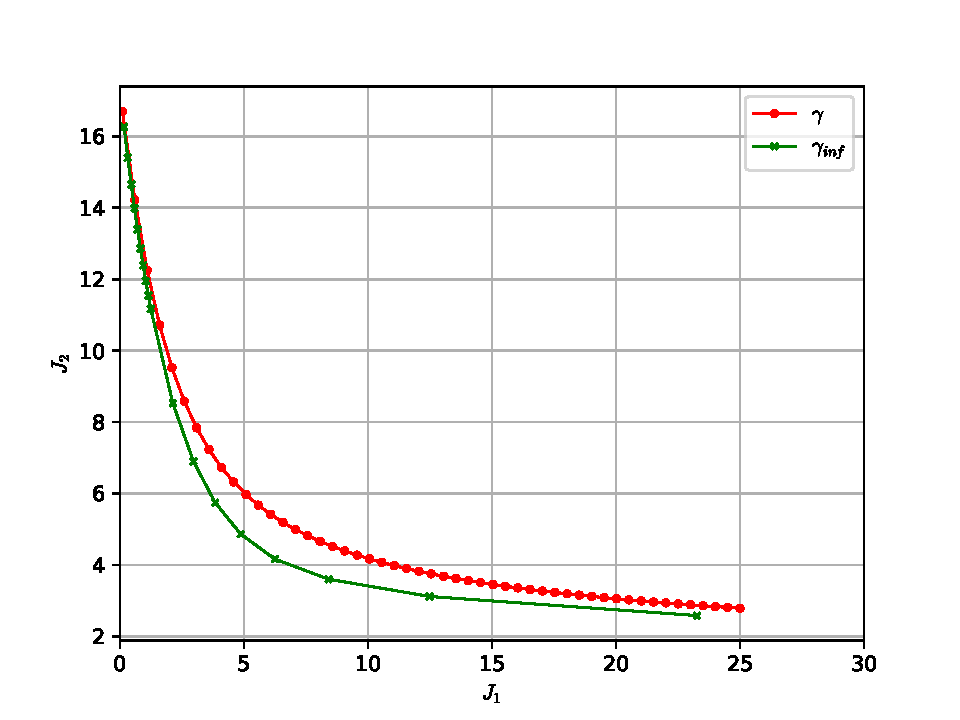
\includegraphics[width=0.75\textwidth]{images/solution.pdf}
    \caption{Парето-границы в задаче виброизоляции при \(n=10\), построенные для
    частично и полностью наблюдаемого состояния}
    \label{fig:pareto}
\end{figure}

Построенная c помощью системы Globalizer описанным ранее способом Парето-граница
показана на рис. \ref{fig:pareto} (кривая \(\gamma\)). При её построении были ограничены
абсолютные значения коэффициентов обратной связи: \(|\theta_i|<10^4\). Сравнивая
кривые \(\gamma_{inf}\) и \(\gamma\), можно сказать, что потеря качества управления при неполной наблюдаемости
и ограниченных коэффициентах обратной связи некритическая.

\section{Заключение}
В ходе работы были получены следующие практические результаты:
\begin{itemize}
  \item реализован метод локальной оптимизации Хука-Дживса (код в приложении \ref{attach1});
  \item в системе Globalizer реализованы различные стратегии использования локального поиска,
  исследована их эффективность;
  \item в рамках Globalizer реализована поддержка смешанного алгоритма глобального поиска,
  а также эффективные структуры данных, необходимые для этого алгоритма (фрагменты кода в приложении \ref{attach2})
  \item был проведён отдельный эксперимент для выяснения возможности практического использования многоуровневых развёрток.
\end{itemize}


\newpage
%\nocite{*}
\addcontentsline{toc}{section}{Список литературы}
\printbibliography
\newpage
\section{Приложения}
\subsection{Приложение 1}
\label{attach1}

\begin{lstlisting}[frame=single]
#ifndef OPTIMIZER_ALGORITHM_UNCONSTRAINED_HPP
#define OPTIMIZER_ALGORITHM_UNCONSTRAINED_HPP

#include "OptimizerCoreGlobal.hpp"
#include "OptimizerTask.hpp"
#include "OptimizerSolution.hpp"
#include "OptimizerFunction.hpp"
#include "OptimizerDataStructures.hpp"
#include "OptimizerSolution.hpp"
#include "OptimizerResult.hpp"
#include "OptimizerSearchSequence.hpp"

#include <set>

namespace optimizercore
{

  class EXPORT_API OptimizerAlgorithmUnconstrained final
  {

  private:

    bool mLocalMixType;
    bool mIsAlgorithmMemoryAllocated;
    bool mIsParamsInitialized;
    bool mIsTaskInitialized;
    bool mNeedLocalVerification;

    int mNumberOfThreads;
    int mLocalStartIterationNumber;
    int mMaxNumberOfIterations;
    int mMapTightness;
    int mMethodDimension;
    int mAlpha;
    int mLocalMixParameter;
    int mMapType;

    OptimizerSpaceTransformation mSpaceTransform;
    OptimizerFunction *mTargetFunction;
    OptimizerFunctionPtr mTargetFunctionSmartPtr;

    OptimizerInterval *mIntervalsForTrials;
    std::set<OptimizerTrialPoint> mSearchInformationStorage;
    OptimizerTrialPoint mOptimumEvaluation, *mNextTrialsPoints;

    LocalTuningMode mLocalTuningMode;

    double mGlobalM, mZ, eps, r, mMaxIntervalNorm;
    double **mNextPoints;

    void AllocMem();
    void InitializeInformationStorage();
    void UpdateGlobalM(std::set<OptimizerTrialPoint>::iterator&);
    int UpdateRanks(bool isLocal);
    bool InsertNewTrials(int trailsNumber);
    OptimizerSolution DoLocalVerification(OptimizerSolution startPoint);

  public:
    OptimizerAlgorithmUnconstrained();
    ~OptimizerAlgorithmUnconstrained();

    void SetTask(OptimizerFunctionPtr function,
      OptimizerSpaceTransformation spaceTransform);
    void SetThreadsNum(int num);
    void SetParameters(OptimizerParameters params);

    OptimizerResult StartOptimization(const double* xOpt,
      StopCriterionType stopType);

    double GetLipschitzConst() const;
    OptimizerSearchSequence GetSearchSequence() const;

  };
}
#endif
\end{lstlisting}
\begin{lstlisting}[frame=single]
  #include "OptimizerAlgorithmUnconstrained.hpp"
  #include "HookeJeevesLocalMethod.hpp"

  #include <cassert>
  #include <algorithm>

  using namespace optimizercore;
  using namespace optimizercore::utils;

  OptimizerAlgorithmUnconstrained::OptimizerAlgorithmUnconstrained()
  {
    mIsAlgorithmMemoryAllocated = false;

    mLocalStartIterationNumber = 1;
    mNumberOfThreads = 1;
    mMaxNumberOfIterations = 5000;
    mNextPoints = nullptr;
    mNextTrialsPoints = nullptr;
    mIntervalsForTrials = nullptr;
    r = 2;
    mLocalTuningMode = LocalTuningMode::None;

    mIsTaskInitialized = false;
    mIsParamsInitialized = false;
  }

  void OptimizerAlgorithmUnconstrained::SetTask(OptimizerFunctionPtr function,
    OptimizerSpaceTransformation spaceTransform)
  {
    assert(function);

    mTargetFunctionSmartPtr = function;
    mTargetFunction = function.get();
    mSpaceTransform = spaceTransform;

    mIsTaskInitialized = true;
  }

  OptimizerSearchSequence OptimizerAlgorithmUnconstrained::GetSearchSequence() const
  {
    return OptimizerSearchSequence(mSearchInformationStorage, mMethodDimension,
      static_cast<MapType> (mMapType), mMapTightness, mSpaceTransform);
  }

  double OptimizerAlgorithmUnconstrained::GetLipschitzConst() const
  {
    return mGlobalM;
  }

  void OptimizerAlgorithmUnconstrained::SetParameters(OptimizerParameters params)
  {
    assert(params.algDimention);
    assert(params.eps > 0);
    assert(params.localAlgStartIterationNumber > 0);
    assert(params.mapTightness > 5 && params.mapTightness <= 20);
    assert(params.maxIterationsNumber > 0);
    assert(params.localMixParameter >= 0 && params.localMixParameter <= 20);
    assert(params.r != nullptr);
    assert(params.numberOfThreads > 0);
    assert(params.reserves != nullptr);
    assert(params.numberOfMaps > 0);

    mLocalStartIterationNumber = params.localAlgStartIterationNumber;
    eps = params.eps;
    if (params.localMixParameter <= 10)	{
      mLocalMixParameter = params.localMixParameter;
      mLocalMixType = true;
    }
    else	{
      mLocalMixParameter = 20 - params.localMixParameter;
      mLocalMixType = false;
    }
    mNeedLocalVerification = params.localVerification;
    mAlpha = params.localExponent;
    mMethodDimension = params.algDimention;
    mMapTightness = params.mapTightness;
    mMapType = static_cast<int>(params.mapType);
    mMaxNumberOfIterations = params.maxIterationsNumber;
    mLocalTuningMode = params.localTuningMode;
    r = *params.r;
    if (mNextPoints)
      utils::DeleteMatrix(mNextPoints, mNumberOfThreads);
    mNextPoints = utils::AllocateMatrix<double>(mNumberOfThreads, mMethodDimension);
    this->SetThreadsNum(params.numberOfThreads);

    mIsParamsInitialized = true;
  }

  void OptimizerAlgorithmUnconstrained::InitializeInformationStorage()
  {
    if (!mIsAlgorithmMemoryAllocated){
      AllocMem();
      mIsAlgorithmMemoryAllocated = true;
    }

    mZ = HUGE_VAL;
    mGlobalM = 1;
    mMaxIntervalNorm = 0;

    mSearchInformationStorage.clear();

    mapd(0.0, mMapTightness, mNextPoints[0], mMethodDimension, mMapType);
    mSpaceTransform.Transform(mNextPoints[0], mNextPoints[0]);
    mSearchInformationStorage.emplace(0.0, mTargetFunction->Calculate(mNextPoints[0]), 0);

    mapd(1.0, mMapTightness, mNextPoints[0], mMethodDimension, mMapType);
    mSpaceTransform.Transform(mNextPoints[0], mNextPoints[0]);
    mSearchInformationStorage.emplace(1.0, mTargetFunction->Calculate(mNextPoints[0]), 0);
  }

  bool OptimizerAlgorithmUnconstrained::InsertNewTrials(int trailsNumber)
  {
    bool storageInsertionError;
    if (mMapType == 3)
    {
      int preimagesNumber = 0;
      double preimages[32];
      for (int i = 0; i < trailsNumber; i++)
      {
        invmad(mMapTightness, preimages, 32,
          &preimagesNumber, mNextPoints[i], mMethodDimension, 4);
        for (int k = 0; k < preimagesNumber; k++)
        {
          mNextTrialsPoints[i].x = preimages[k];
          auto insertionResult =
            mSearchInformationStorage.insert(mNextTrialsPoints[i]);

          if (!(storageInsertionError = insertionResult.second))
            break;

          UpdateGlobalM(insertionResult.first);
        }
      }
    }
    else
      for (int i = 0; i < trailsNumber; i++)
      {
        auto insertionResult =
          mSearchInformationStorage.insert(mNextTrialsPoints[i]);

        if (!(storageInsertionError = insertionResult.second))
          break;

        UpdateGlobalM(insertionResult.first);
      }
    return storageInsertionError;
  }

  OptimizerResult OptimizerAlgorithmUnconstrained::StartOptimization(
    const double* a, StopCriterionType stopType)
  {
    assert(mIsParamsInitialized && mIsTaskInitialized);
    assert(mSpaceTransform.GetDomainDimension() == mMethodDimension);

    InitializeInformationStorage();

    double *y;
    bool stop = false;
    int iterationsCount = 0,
      currentThrNum = 1, ranksUpdateErrCode;

    mNextTrialsPoints[0].x = 0.5;
    mapd(mNextTrialsPoints[0].x, mMapTightness, mNextPoints[0],
      mMethodDimension, mMapType);
    mSpaceTransform.Transform(mNextPoints[0], mNextPoints[0]);

    while (iterationsCount < mMaxNumberOfIterations && !stop)	{
      iterationsCount++;

  #pragma omp parallel for num_threads(currentThrNum)
      for (int i = 0; i < currentThrNum; i++)	{
        mNextTrialsPoints[i].val = mTargetFunction->Calculate(mNextPoints[i]);
        if (mMapType == 3)
          mSpaceTransform.InvertTransform(mNextPoints[i], mNextPoints[i]);
  #pragma omp critical
        if (mNextTrialsPoints[i].val < mZ)
          mZ = mNextTrialsPoints[i].val;
      }

      if (!InsertNewTrials(currentThrNum))
        break;

      if (iterationsCount >= mLocalStartIterationNumber)	{
        if (iterationsCount % (12 - mLocalMixParameter) == 0
          && mLocalMixParameter > 0)
          ranksUpdateErrCode = UpdateRanks(mLocalMixType);
        else
          ranksUpdateErrCode = UpdateRanks(!mLocalMixType);
      }
      else
        ranksUpdateErrCode = UpdateRanks(false);

      if (iterationsCount >= mNumberOfThreads + 10)
        currentThrNum = mNumberOfThreads;

      for (int i = 0; i < currentThrNum && !stop; i++)	{
        OptimizerTrialPoint left = mIntervalsForTrials[i].left;
        OptimizerTrialPoint right = mIntervalsForTrials[i].right;

        mNextTrialsPoints[i].x = (left.x + right.x) / 2
          - sgn(right.val - left.val)*pow(fabs(right.val - left.val)
          / mIntervalsForTrials[i].localM, mMethodDimension) / (2 * r);

        mapd(mNextTrialsPoints[i].x, mMapTightness, mNextPoints[i],
          mMethodDimension, mMapType);
        mSpaceTransform.Transform(mNextPoints[i], mNextPoints[i]);

        y = mNextPoints[i];

        if (stopType == StopCriterionType::OptimalPoint)	{
          if (NormNDimMax(y, a, mMethodDimension) < eps)	{
            stop = true;
            mOptimumEvaluation = mNextTrialsPoints[i];
          }
        }
        else	{
          if (pow(right.x - left.x, 1.0 / mMethodDimension) < eps)	{
            stop = true;
            mOptimumEvaluation = mNextTrialsPoints[i];
          }
        }
      }
    }

    mOptimumEvaluation.val = mTargetFunction->Calculate(y);
    mSearchInformationStorage.insert(mOptimumEvaluation);

    if (stopType == StopCriterionType::Precision)
      mOptimumEvaluation = *std::min_element(mSearchInformationStorage.begin(),
        mSearchInformationStorage.cend(),
        [](OptimizerTrialPoint p1, OptimizerTrialPoint p2)
      {
        return p1.val < p2.val;
      });

    mapd(mOptimumEvaluation.x, mMapTightness, y, mMethodDimension, mMapType);
    mSpaceTransform.Transform(y, y);

    SharedVector optPoint(new double[mMethodDimension], array_deleter<double>());
    std::memcpy(optPoint.get(), y, mMethodDimension*sizeof(double));

    OptimizerSolution solution(iterationsCount, mOptimumEvaluation.val,
      mOptimumEvaluation.x, mMethodDimension, optPoint);

    if (mNeedLocalVerification)
      return OptimizerResult(DoLocalVerification(solution));
    else
      return OptimizerResult(solution);
  }
  OptimizerSolution OptimizerAlgorithmUnconstrained::DoLocalVerification(OptimizerSolution startSolution)
  {
    OptimizerFunctionPtr *functions = new OptimizerFunctionPtr[1];
    functions[0] = mTargetFunctionSmartPtr;

    OptimizerTask localTask(std::shared_ptr<OptimizerFunctionPtr>(functions,
      utils::array_deleter<OptimizerFunctionPtr>()),
      0, mMethodDimension, mSpaceTransform.GetLeftDomainBound(),
      mSpaceTransform.GetRightDomainBound());

    localoptimizer::HookeJeevesLocalMethod localMethod;
    localMethod.SetEps(eps / 100);
    localMethod.SetInitialStep(2 * eps);
    localMethod.SetProblem(localTask);
    localMethod.SetStepMultiplier(2);
    localMethod.SetStartPoint(startSolution.GetOptimumPoint().get(),
      localTask.GetTaskDimension());

    SharedVector localOptimum(new double[mMethodDimension], array_deleter<double>());
    localMethod.StartOptimization(localOptimum.get());
    double bestLocalValue = mTargetFunction->Calculate(localOptimum.get());

    if (startSolution.GetOptimumValue() > bestLocalValue)
      return OptimizerSolution(startSolution.GetIterationsCount(),
      bestLocalValue, 0.5, mMethodDimension, localOptimum);

    return startSolution;
  }
  void OptimizerAlgorithmUnconstrained::SetThreadsNum(int num)
  {
    if (num > 0 && num < 100)
    {
      if (mNextPoints != nullptr)
        utils::DeleteMatrix(mNextPoints, mNumberOfThreads);
      mNumberOfThreads = num;
      if (mNextTrialsPoints)
        delete[] mNextTrialsPoints;
      if (mIntervalsForTrials)
        delete[] mIntervalsForTrials;
      mIntervalsForTrials = new OptimizerInterval[num];
      mNextTrialsPoints = new OptimizerTrialPoint[num];
      mNextPoints = utils::AllocateMatrix<double>(
        mNumberOfThreads, mMethodDimension);
    }
  }
  OptimizerAlgorithmUnconstrained::~OptimizerAlgorithmUnconstrained()
  {
    if (mIntervalsForTrials)
      delete[] mIntervalsForTrials;
    if (mNextPoints)
      utils::DeleteMatrix(mNextPoints, mNumberOfThreads);
    if (mNextTrialsPoints)
      delete[] mNextTrialsPoints;
    if (mIsAlgorithmMemoryAllocated)
    {
    }
  }
  void OptimizerAlgorithmUnconstrained::UpdateGlobalM(
    std::set<OptimizerTrialPoint>::iterator& newPointIt)
  {
    double max = mGlobalM;
    if (max == 1) max = 0;


    auto leftPointIt = newPointIt;
    auto rightPointIt = newPointIt;
    --leftPointIt;
    ++rightPointIt;

    double leftIntervalNorm = pow(newPointIt->x - leftPointIt->x, 1.0 / mMethodDimension);
    double rightIntervalNorm = pow(rightPointIt->x - newPointIt->x, 1.0 / mMethodDimension);


    max = fmax(fmax(fabs(newPointIt->val - leftPointIt->val) / leftIntervalNorm,
      fabs(rightPointIt->val - newPointIt->val) /	rightIntervalNorm), max);


    mMaxIntervalNorm = 0;
    auto currentPointIt = mSearchInformationStorage.begin();
    auto nextPointIt = currentPointIt;
    ++nextPointIt;

    while (nextPointIt != mSearchInformationStorage.cend())
    {
      if (mLocalTuningMode != LocalTuningMode::None)
        mMaxIntervalNorm = fmax(
          pow(nextPointIt->x - currentPointIt->x, 1.0 / mMethodDimension),
          mMaxIntervalNorm);

      ++currentPointIt;
      ++nextPointIt;
    }
    if (max != 0)
      mGlobalM = max;
    else
      mGlobalM = 1;
  }
  int OptimizerAlgorithmUnconstrained::UpdateRanks(bool isLocal)
  {
    double dx, curr_rank, mu1 = -HUGE_VAL, localM = mGlobalM;
    double localMConsts[3];

    for (int i = 0; i < mNumberOfThreads; i++)
      mIntervalsForTrials[i].R = -HUGE_VAL;

    auto leftIt = mSearchInformationStorage.begin();
    auto rightIt = mSearchInformationStorage.begin();
    ++rightIt;

    int storageSize = mSearchInformationStorage.size();

    for (int j = 0; j < storageSize - 1; j++)
    {
      dx = pow(rightIt->x - leftIt->x, 1.0 / mMethodDimension);

      if (dx == 0)
        return 1;

      if (mLocalTuningMode != LocalTuningMode::None)	{
        std::set<OptimizerTrialPoint>::iterator rightRightIt = rightIt;

        if (j > 0 && j < storageSize - 2)	{
          ++rightRightIt;

          std::swap(localMConsts[0], localMConsts[1]);
          std::swap(localMConsts[1], localMConsts[2]);

          localMConsts[2] = fabs(rightRightIt->val - rightIt->val)
            / pow(rightRightIt->x - rightIt->x, 1.0 / mMethodDimension);

          mu1 = fmax(fmax(localMConsts[0], localMConsts[1]), localMConsts[2]);
        }
        else if (j == 0)	{
          ++rightRightIt;

          localMConsts[1] = fabs(rightIt->val - leftIt->val) / dx;
          localMConsts[2] = fabs(rightRightIt->val - rightIt->val) /
            pow(rightRightIt->x - rightIt->x, 1.0 / mMethodDimension);
          mu1 = fmax(localMConsts[1], localMConsts[2]);
        }
        else
          mu1 = fmax(localMConsts[1], localMConsts[2]);

        double mu2 = mGlobalM*dx / mMaxIntervalNorm;

        if (mLocalTuningMode == LocalTuningMode::Maximum)	{
          localM = fmax(fmax(mu1, mu2), 0.01);
        }
        else// LocalTuningMode::Adaptive
          localM = fmax(mu1 / r + (1 - 1 / r)*mGlobalM, 0.01);
          //localM = fmax(mu1*(1 - dx / mMaxIntervalNorm) + mu2, 0.01);
          //localM = fmax(mu1*mMConvolution + (1 - mMConvolution)*mu2, 0.01);
      }

      curr_rank = dx + Pow2((rightIt->val - leftIt->val) / (r * localM)) / dx
        - 2 * (rightIt->val + leftIt->val - 2 * mZ) / (r * localM);
      if (isLocal)
        curr_rank /= sqrt((rightIt->val - mZ)*
        (leftIt->val - mZ)) / localM + pow(1.5, -mAlpha);

      if (curr_rank > mIntervalsForTrials[mNumberOfThreads - 1].R)
      {
        OptimizerInterval newInterval(
          OptimizerTrialPoint(*leftIt),
          OptimizerTrialPoint(*rightIt), curr_rank, localM);
        for (int i = 0; i < mNumberOfThreads; i++)
          if (mIntervalsForTrials[i].R < newInterval.R)
            std::swap(mIntervalsForTrials[i], newInterval);
      }
      ++leftIt;
      ++rightIt;
    }
    return 0;
  }
  void OptimizerAlgorithmUnconstrained::AllocMem()
  {
  }
\end{lstlisting}

\subsection{Приложение 2}
\label{attach2}
\begin{lstlisting}[frame=single]
#ifndef __OPTMAL_CONTROL_PROBLEM_H__
#define __OPTMAL_CONTROL_PROBLEM_H__

#include "problem_interface.h"
#include "optimal_problem_base.h"

#include <Eigen/Dense>
#include <string>

class TOptimalControlProblem : public IProblem
{
protected:

  OptimalControlProblemBase* mPProblemImpl;
  int mDimension;
  bool mIsInitialized;
  std::string mConfigPath;

public:
  TOptimalControlProblem();
  virtual int SetConfigPath(const std::string& configPath);
  virtual int SetDimension(int dimension);
  virtual int GetDimension() const;
  virtual int Initialize();

  virtual void GetBounds(double* lower, double *upper);
  virtual int GetOptimumValue(double& value) const;
  virtual int GetOptimumPoint(double* x) const;

  virtual int GetNumberOfFunctions() const;
  virtual int GetNumberOfConstraints() const;
  virtual int GetNumberOfCriterions() const;

  virtual double CalculateFunctionals(const double* x, int fNumber);

  ~TOptimalControlProblem();
};

extern "C" LIB_EXPORT_API IProblem* create();
extern "C" LIB_EXPORT_API void destroy(IProblem* ptr);
#endif
\end{lstlisting}
\begin{lstlisting}[frame=single]
#include "optimalControl.h"
#include "test_problems.h"
#include "problemA.h"
#include "problemB.h"
#include "pugixml.hpp"

#include <string>
#include <stdexcept>

TOptimalControlProblem::TOptimalControlProblem()
{
  mIsInitialized = false;
}

int TOptimalControlProblem::SetConfigPath(const std::string& configPath)
{
  mConfigPath = std::string(configPath);
  return IProblem::OK;
}

int TOptimalControlProblem::SetDimension(int dimension)
{
    return IProblem::OK;
}

int TOptimalControlProblem::GetDimension() const
{
  return mDimension;
}

int TOptimalControlProblem::Initialize()
{
  if (mIsInitialized == false)
  {
    mIsInitialized = true;

    pugi::xml_document doc;
    pugi::xml_parse_result result = doc.load_file(mConfigPath.c_str());
    if (result.status != pugi::status_ok)
      return IProblem::ERROR;

    pugi::xml_node config = doc.child("config");
    std::string problemName = config.child("problem_name").child_value();
    double secondCriterionLevel = 0.;
    double lambda = 0.;
    int dimension = 0;
    try  {
      secondCriterionLevel = std::stod(config.child("S").child_value());
      lambda = std::stod(config.child("lambda").child_value());
      dimension = std::stoi(config.child("N").child_value());
    }
    catch (std::invalid_argument& exp)  {
      return IProblem::ERROR;
    }

    if (problemName == std::string("v"))
      mPProblemImpl = new VibroisolationProblem();
    else if (problemName == std::string("od"))
      mPProblemImpl = new OscillationDampingProblem();
    else if (problemName == std::string("a2d"))
      mPProblemImpl = new ProblemA2d(secondCriterionLevel);
    else if (problemName == std::string("a3d"))
      mPProblemImpl = new ProblemA3d(secondCriterionLevel);
    else if (problemName == std::string("bNd") && dimension == 2)
      mPProblemImpl = new ProblemB2d(secondCriterionLevel);
    else if (problemName == std::string("bNd"))
      mPProblemImpl = new ProblemB(secondCriterionLevel, dimension);
    else if (problemName == std::string("bNdC"))
      mPProblemImpl = new ProblemBConvolved(lambda, dimension);
    else
      return IProblem::ERROR;

    mDimension = mPProblemImpl->GetDimension();

    return IProblem::OK;
  }
  else
    return IProblem::ERROR;
}

void TOptimalControlProblem::GetBounds(double* lower, double *upper)
{
  if (mIsInitialized)
    mPProblemImpl->GetBounds(lower, upper);
}

int TOptimalControlProblem::GetOptimumValue(double& value) const
{
  return IProblem::UNDEFINED;
}

int TOptimalControlProblem::GetOptimumPoint(double* point) const
{
  return IProblem::UNDEFINED;
}

int TOptimalControlProblem::GetNumberOfFunctions() const
{
  return mPProblemImpl->GetNumberOfFunctions();
}

int TOptimalControlProblem::GetNumberOfConstraints() const
{
  return mPProblemImpl->GetNumberOfConstraints();
}

int TOptimalControlProblem::GetNumberOfCriterions() const
{
  return 1;
}

// ------------------------------------------------------------------------------------------------
double TOptimalControlProblem::CalculateFunctionals(const double* x, int fNumber)
{
  return mPProblemImpl->CalculateFunctionals(x, fNumber);
}

TOptimalControlProblem::~TOptimalControlProblem()
{
  if(mIsInitialized)
  {
    mPProblemImpl->PrintFinalMessage();
    delete mPProblemImpl;
  }
}

LIB_EXPORT_API IProblem* create()
{
  return new TOptimalControlProblem();
}

LIB_EXPORT_API void destroy(IProblem* ptr)
{
  delete ptr;
}
\end{lstlisting}
\begin{lstlisting}[frame=single]
#ifndef OPTIMAL_CONTROL_BASE_H
#define OPTIMAL_CONTROL_BASE_H

#ifndef EIGEN_DONT_PARALLELIZE
#define EIGEN_DONT_PARALLELIZE
#endif

#include <Eigen/Dense>
#include <vector>

class OptimalControlProblemBase
{
protected:
  int mDimension;
  int n_x;
  int n_v;
  int n_u;
  std::vector<int> n_k;

  Eigen::MatrixXd A;
  Eigen::MatrixXd B_u;
  Eigen::MatrixXd B_v;
  Eigen::MatrixXd* YVecs;
  std::vector<Eigen::MatrixXd> CMatrices;
  std::vector<Eigen::MatrixXd> DMatrices;

  double mZeroConstraintOffset;
  double mS;

  virtual Eigen::RowVectorXd getTheta(const double* x);
  virtual double CalculateCriterionValue(const Eigen::RowVectorXd& theta, int fNumber);

public:
  OptimalControlProblemBase();
  virtual ~OptimalControlProblemBase();
  virtual void GetBounds(double* lower, double *upper) const = 0;
  virtual double CalculateFunctionals(const double* x, int fNumber);
  int GetDimension() const { return mDimension; }
  virtual int GetNumberOfConstraints() const { return 2; }
  virtual int GetNumberOfFunctions() const { return 3; }
  virtual void PrintFinalMessage() {}
};

#endif
\end{lstlisting}
\begin{lstlisting}[frame=single]
#include "optimal_problem_base.h"

#define _USE_MATH_DEFINES
#include <math.h>
#include <algorithm>
#include <omp.h>

using namespace Eigen;

OptimalControlProblemBase::OptimalControlProblemBase()
{
  YVecs = new MatrixXd[omp_get_num_procs()];
}

OptimalControlProblemBase::~OptimalControlProblemBase()
{
  delete[] YVecs;
}

RowVectorXd OptimalControlProblemBase::getTheta(const double* x)
{
  return Map<const RowVectorXd>(x, mDimension);
}

MatrixXd buildVectorizationMatrix(const MatrixXd& A)
{
  size_t n = A.cols();

  MatrixXd E = MatrixXd::Identity(n, n);
  MatrixXd S(n*n, n*n);

  for(size_t i = 0; i < n; i++)
    for(size_t j = 0; j < n; j++)
    {
      if(i != j)
        S.block(i*n, j*n, n, n) = A.coeff(i, j)*E;
      else
        S.block(i*n, j*n, n, n) = A + A.coeff(i, j)*E;
    }

  return S;
}

double OptimalControlProblemBase::CalculateCriterionValue(const Eigen::RowVectorXd& theta, int fNumber)
{
  Map<MatrixXd> Y(YVecs[omp_get_thread_num()].data(), A.cols(), A.rows());

  double value = -HUGE_VAL;
  size_t cRows = CMatrices[fNumber].rows();
  for (size_t i = 0; i < cRows; i++)
  {
    RowVectorXd currentVector = CMatrices[fNumber].row(i) + DMatrices[fNumber].row(i)*theta;
    double dotProd = (currentVector*Y).dot(currentVector.transpose());
    value = std::max(value, dotProd);
  }
  return value;
}

double OptimalControlProblemBase::CalculateFunctionals(const double* x, int fNumber)
{
  RowVectorXd theta = getTheta(x);

  if (fNumber == 0)
  {
    MatrixXd Atheta = A + B_u*theta;

    EigenSolver<MatrixXd> eigenSolver(Atheta, false);
    MatrixXcd eigenvalues = eigenSolver.eigenvalues();
    double maxReal = -HUGE_VAL;
    for (int i = 0; i < Atheta.cols(); i++)
      maxReal = std::max(maxReal, eigenvalues.coeff(i).real());

    return maxReal + mZeroConstraintOffset;
  }
  else if (fNumber == 1)
  {
    MatrixXd Atheta = A + B_u*theta;
    MatrixXd S = buildVectorizationMatrix(Atheta);
    MatrixXd rhs = -B_v*B_v.transpose();
    Map<VectorXd> rhsMap(rhs.data(), rhs.size());
    YVecs[omp_get_thread_num()] = S.partialPivLu().solve(rhsMap);
  }

  fNumber--;
  double offset = fNumber == 0 ? -mS : 0.;
  double value = CalculateCriterionValue(theta, fNumber);

  return sqrt(value) + offset;
}
\end{lstlisting}
\begin{lstlisting}[frame=single]
#pragma once
#include "optimal_problem_base.h"

#define _USE_MATH_DEFINES
#include <math.h>
#include <algorithm>
#include <iostream>

using namespace Eigen;
using Eigen::internal::BandMatrix;

class ProblemB_Common : public OptimalControlProblemBase
{
public:
  ProblemB_Common(double S)
  {
    double beta = 0.1;

    int n = 10;

    n_x = 2*n;
    n_v = 1;
    n_u = 1;
    n_k.resize(2);
    n_k[0] = n_k[1] = 1;

    CMatrices.resize(2);
    DMatrices.resize(2);

    A.resize(n_x, n_x);
    A.topLeftCorner(n, n).setZero();
    A.topRightCorner(n, n).setIdentity();

    BandMatrix<double> K(n, n, 1, 1);
    K.diagonal().setConstant(2.);
    K.diagonal(-1).setConstant(-1.);
    K.diagonal(1).setConstant(-1.);
    K.diagonal()(0) = 1.;
    K.diagonal()(n - 1) = 1.;

    A.bottomLeftCorner(n, n) = -K.toDenseMatrix();
    A.bottomRightCorner(n, n) = -beta*K.toDenseMatrix();

    B_v.resize(n_x, 1);
    B_v.col(0).head(n).setZero();
    B_v.col(0).tail(n).setOnes();

    B_u = VectorXd::Zero(n_x);
    B_u(n, 0) = 1.;

    CMatrices[0].resize(1, n_x);
    CMatrices[0].setZero();
    CMatrices[0](0, 0) = 1.;

    CMatrices[1].resize(n - 1, n_x);

    for(size_t i = 0; i < n - 1; i++)
    {
      CMatrices[1].row(i).setZero();
      CMatrices[1].row(i)(i) = -1.;
      CMatrices[1].row(i)(i + 1) = 1.;
    }

    DMatrices[0].resize(1, 1); DMatrices[0] << 0;

    DMatrices[1].resize(n - 1, 1);
    DMatrices[1].setZero();

    mS = S;
    mZeroConstraintOffset = 0.;
  }

  int GetNumberOfConstraints() const { return 2; }
};

class ProblemB : public ProblemB_Common
{
public:
  ProblemB(double S, int dimension) : ProblemB_Common(S)
  {
    mDimension = dimension;//shoud be > 2
  }

  void GetBounds(double* lower, double *upper) const
  {
    for (int i = 0; i < mDimension; i++)
    {
      lower[i] = -10000.;
      upper[i] = -0.01;
    }

    for (int i = 2; i < mDimension; i++)
    {
      upper[i] = 10000.;
    }
  }

  RowVectorXd getTheta(const double* x)
  {
    RowVectorXd theta(n_x);
    theta.setZero();

    theta(0) = x[0] - x[2];
    for (int i = 1; i < mDimension - 2; i++)
        theta(i) = x[i + 1] - x[i + 2];
    theta(mDimension - 2) = x[mDimension - 1];
    theta(n_x / 2) = x[1];

    return theta;
  }
};

class ProblemB2d : public ProblemB_Common
{
public:
  ProblemB2d(double S) : ProblemB_Common(S)
  {
    mDimension = 2;
  }

  void GetBounds(double* lower, double *upper) const
  {
    for (int i = 0; i < mDimension; i++)
    {
      lower[i] = -70.;
      upper[i] = -0.01;
    }
    lower[0] = -20.;
  }

  RowVectorXd getTheta(const double* x)
  {
    RowVectorXd theta(n_x);
    theta.setZero();
    theta(0) = x[0];
    theta(n_x / 2) = x[1];

    return theta;
  }
};
\end{lstlisting}
\begin{lstlisting}[frame=single]
#ifndef __OPTMAL_CONTROL_TEST_IMPL_H__
#define __OPTMAL_CONTROL_TEST_IMPL_H__

#include "optimal_problem_base.h"

class VibroisolationProblem : public OptimalControlProblemBase
{
public:
  VibroisolationProblem()
  {
    n_x = 2;
    n_v = 1;
    n_u = 1;
    n_k.resize(2);
    n_k[0] = n_k[1] = 1;

    CMatrices.resize(2);
    DMatrices.resize(2);

    A.resize(2, 2); A << 0, 1, 0, 0;
    B_u.resize(2, 1); B_u << 0, 1;
    B_v = B_u;

    CMatrices[0].resize(1, 2); CMatrices[0] << 1, 0;
    CMatrices[1].resize(1, 2); CMatrices[1] << 0, 0;

    DMatrices[0].resize(1, 1); DMatrices[0] << 0;
    DMatrices[1].resize(1, 1); DMatrices[1] << 1;
    mDimension = n_x;
    mZeroConstraintOffset = 0.;
    mS = 1.;
  }

  int GetNumberOfConstraints() const { return 2; }

  void GetBounds(double* lower, double *upper) const
  {
    for (int i = 0; i < mDimension; i++)
    {
      upper[i] = -0.2;
      lower[i] = -2.0;
    }
  }
};

class OscillationDampingProblem : public OptimalControlProblemBase
{
public:
  OscillationDampingProblem()
  {
    double beta = 0.1;
    n_x = 4;
    n_v = 1;
    n_u = 1;
    n_k.resize(2);
    n_k[0] = n_k[1] = 1;

    CMatrices.resize(2);
    DMatrices.resize(2);

    A.resize(4, 4);
    A << 0, 0, 1, 0,
      0, 0, 0, 1,
      -2, 1, -2*beta, beta,
      1, -1, beta, -beta;

    B_u.resize(4, 1); B_u << 0, 0, 0, 1;
    B_v.resize(4, 1); B_v << 0, 0, 1, 1;

    CMatrices[0].resize(2, 4);
    CMatrices[0] << 1, 0, 0, 0,
      -1, 1, 0, 0;
    CMatrices[1].resize(1, 4); CMatrices[1] << 0, 0, 0, 0;

    DMatrices[0].resize(2, 1); DMatrices[0] << 0, 0;
    DMatrices[1].resize(1, 1); DMatrices[1] << 1;
    mDimension = n_x;
    mZeroConstraintOffset = 0.02;
    mS = 1.;
  }

  int GetNumberOfConstraints() const
  {
    return 2;
  }

  void GetBounds(double* lower, double *upper) const
  {
    for (int i = 0; i < mDimension; i++)
    {
      upper[i] = 1;
      lower[i] = -2.0;
    }
  }
};
#endif
\end{lstlisting}

\subsection{Приложение 3}
\label{attach3}
\begin{lstlisting}[frame=single]
#ifndef __LOCALMETHOD_H__
#define __LOCALMETHOD_H__

#include "parameters.h"
#include "task.h"
#include "data.h"
#include "common.h"
#include <vector>

#define MAX_LOCAL_TRIALS_NUMBER 10000

class TLocalMethod
{
protected:

  int mDimension;
  int mConstraintsNumber;
  int mTrialsCounter;
  int mMaxTrial;

  TTrial mBestPoint;
  std::vector<TTrial> mSearchSequence;
  TTask* mPTask;

  bool mIsLogPoints;

  double mEps;
  double mStep;
  double mStepMultiplier;

  OBJECTIV_TYPE *mFunctionsArgument;
  OBJECTIV_TYPE *mStartPoint;
  OBJECTIV_TYPE* mCurrentPoint;
  OBJECTIV_TYPE* mCurrentResearchDirection;
  OBJECTIV_TYPE* mPreviousResearchDirection;

  double MakeResearch(OBJECTIV_TYPE*);
  void DoStep();
  double EvaluateObjectiveFunctiuon(const OBJECTIV_TYPE*);

public:

  TLocalMethod();
  TLocalMethod(TParameters _params, TTask* _pTask, TTrial _startPoint, bool logPoints = false);
  ~TLocalMethod();

  void SetEps(double);
  void SetInitialStep(double);
  void SetStepMultiplier(double);
  void SetMaxTrials(int);

  int GetTrialsCounter() const;
  std::vector<TTrial> GetSearchSequence() const;

  TTrial StartOptimization();
};

#endif //__LOCALMETHOD_H__
\end{lstlisting}

\begin{lstlisting}[frame=single]
#include "local_method.h"
#include <cmath>
#include <cstring>
#include <algorithm>

TLocalMethod::TLocalMethod(TParameters _params, TTask* _pTask, TTrial _startPoint, bool logPoints)
{
  mEps = _params.Epsilon / 100;
  if (mEps > 0.0001)
    mEps = 0.0001;
  mBestPoint = _startPoint;
  mStep = _params.Epsilon * 2;
  mStepMultiplier = 2;
  mTrialsCounter = 0;
  mIsLogPoints = logPoints;

  mPTask = _pTask;

  mDimension = mPTask->GetN() - mPTask->GetFixedN();
  mConstraintsNumber = mPTask->GetNumOfFunc() - 1;

  mStartPoint = new OBJECTIV_TYPE[mDimension];
  std::memcpy(mStartPoint,
    _startPoint.y + mPTask->GetFixedN(),
    mDimension * sizeof(OBJECTIV_TYPE));

  mFunctionsArgument = new OBJECTIV_TYPE[mPTask->GetN()];
  std::memcpy(mFunctionsArgument,
    _startPoint.y,
    mPTask->GetN() * sizeof(OBJECTIV_TYPE));
  mMaxTrial = MAX_LOCAL_TRIALS_NUMBER;
}

TLocalMethod::TLocalMethod() : mPTask(NULL), mStartPoint(NULL),
mFunctionsArgument(NULL), mMaxTrial(MAX_LOCAL_TRIALS_NUMBER)
{
}

TLocalMethod::~TLocalMethod()
{
  if (mStartPoint)
    delete[] mStartPoint;
  if (mFunctionsArgument)
    delete[] mFunctionsArgument;
}

void TLocalMethod::DoStep()
{
  for (int i = 0; i < mDimension; i++)
    mCurrentPoint[i] = (1 + mStepMultiplier)*mCurrentResearchDirection[i] -
    mStepMultiplier*mPreviousResearchDirection[i];
}

TTrial TLocalMethod::StartOptimization()
{
  int k = 0, i = 0;
  bool needRestart = true;
  double currentFValue, nextFValue;
  mTrialsCounter = 0;

  mCurrentPoint = new OBJECTIV_TYPE[mDimension];
  mCurrentResearchDirection = new OBJECTIV_TYPE[mDimension];
  mPreviousResearchDirection = new OBJECTIV_TYPE[mDimension];

  while (mTrialsCounter < mMaxTrial) {
    i++;
    if (needRestart) {
      k = 0;
      std::memcpy(mCurrentPoint, mStartPoint, sizeof(OBJECTIV_TYPE)*mDimension);
      std::memcpy(mCurrentResearchDirection, mStartPoint, sizeof(OBJECTIV_TYPE)*mDimension);
      currentFValue = EvaluateObjectiveFunctiuon(mCurrentPoint);
      needRestart = false;
    }

    std::swap(mPreviousResearchDirection, mCurrentResearchDirection);
    std::memcpy(mCurrentResearchDirection, mCurrentPoint, sizeof(OBJECTIV_TYPE)*mDimension);
    nextFValue = MakeResearch(mCurrentResearchDirection);

    if (currentFValue > nextFValue) {
      DoStep();

      if (mIsLogPoints)
      {
        TTrial currentTrial;
        currentTrial.index = mBestPoint.index;
        currentTrial.FuncValues[currentTrial.index] = nextFValue;
        std::memcpy(currentTrial.y, mFunctionsArgument, sizeof(OBJECTIV_TYPE)*mPTask->GetFixedN());
        std::memcpy(currentTrial.y + mPTask->GetFixedN(), mCurrentPoint, sizeof(OBJECTIV_TYPE)*mDimension);
        mSearchSequence.push_back(currentTrial);
      }
      k++;
      currentFValue = nextFValue;
    }
    else if (mStep > mEps) {
      if (k != 0)
        std::memcpy(mStartPoint, mPreviousResearchDirection, sizeof(OBJECTIV_TYPE)*mDimension);
      else
        mStep /= mStepMultiplier;
      needRestart = true;
    }
    else
      break;
  }

  if (currentFValue < mBestPoint.FuncValues[mConstraintsNumber])
  {
    std::memcpy(mBestPoint.y + mPTask->GetFixedN(),
      mPreviousResearchDirection, sizeof(OBJECTIV_TYPE)*mDimension);
    mBestPoint.FuncValues[mConstraintsNumber] = currentFValue;
    mSearchSequence.push_back(mBestPoint);
  }

  delete[] mCurrentPoint;
  delete[] mPreviousResearchDirection;
  delete[] mCurrentResearchDirection;

  return mBestPoint;
}

double TLocalMethod::EvaluateObjectiveFunctiuon(const OBJECTIV_TYPE* x)
{
  if (mTrialsCounter >= mMaxTrial)
    return HUGE_VAL;

  for (int i = 0; i < mDimension; i++)
    if (x[i] < mPTask->GetA()[mPTask->GetFixedN() + i] ||
      x[i] > mPTask->GetB()[mPTask->GetFixedN() + i])
      return HUGE_VAL;

  std::memcpy(mFunctionsArgument + mPTask->GetFixedN(), x, mDimension * sizeof(OBJECTIV_TYPE));
  for (int i = 0; i <= mConstraintsNumber; i++)
  {
    double value = mPTask->GetFuncs()[i](mFunctionsArgument);
    if (i < mConstraintsNumber && value > 0)
    {
      mTrialsCounter++;
      return HUGE_VAL;
    }
    else if (i == mConstraintsNumber)
    {
      mTrialsCounter++;
      return value;
    }
  }

  return HUGE_VAL;
}

void TLocalMethod::SetEps(double eps)
{
  mEps = eps;
}

void TLocalMethod::SetInitialStep(double value)
{
  mStep = value;
}

void TLocalMethod::SetStepMultiplier(double value)
{
  mStepMultiplier = value;
}

void TLocalMethod::SetMaxTrials(int count)
{
  mMaxTrial = std::min(count, MAX_LOCAL_TRIALS_NUMBER);
}

int TLocalMethod::GetTrialsCounter() const
{
  return mTrialsCounter;
}

std::vector<TTrial> TLocalMethod::GetSearchSequence() const
{
  return mSearchSequence;
}

double TLocalMethod::MakeResearch(OBJECTIV_TYPE* startPoint)
{
  double bestValue = EvaluateObjectiveFunctiuon(startPoint);

  for (int i = 0; i < mDimension; i++)
  {
    startPoint[i] += mStep;
    double rightFvalue = EvaluateObjectiveFunctiuon(startPoint);

    if (rightFvalue > bestValue)
    {
      startPoint[i] -= 2 * mStep;
      double leftFValue = EvaluateObjectiveFunctiuon(startPoint);
      if (leftFValue > bestValue)
        startPoint[i] += mStep;
      else
        bestValue = leftFValue;
    }
    else
      bestValue = rightFvalue;
  }

  return bestValue;
}
\end{lstlisting}

\subsection{Приложение 4}
\label{attach4}
\begin{lstlisting}[frame=single]
#ifndef __DUAL_QUEUE_H__
#define __DUAL_QUEUE_H__

#include "minmaxheap.h"
#include "common.h"
#include "queue_common.h"

class TPriorityDualQueue : public TPriorityQueueCommon
{
protected:
  int MaxSize;
  int CurLocalSize;
  int CurGlobalSize;

  MinMaxHeap< TQueueElement, _less >* pGlobalHeap;
  MinMaxHeap< TQueueElement, _less >* pLocalHeap;

  void DeleteMinLocalElem();
  void DeleteMinGlobalElem();
  void ClearLocal();
  void ClearGlobal();
public:

  TPriorityDualQueue(int _MaxSize = DefaultQueueSize); // _MaxSize must be qual to 2^k - 1
  ~TPriorityDualQueue();

  int GetLocalSize() const;
  int GetSize() const;
  int GetMaxSize() const;
  bool IsLocalEmpty() const;
  bool IsLocalFull() const;
  bool IsEmpty() const;
  bool IsFull() const;

  void Push(double globalKey, double localKey, void *value);
  void PushWithPriority(double globalKey, double localKey, void *value);
  void Pop(double *key, void **value);

  void PopFromLocal(double *key, void **value);

  void Clear();
  void Resize(int size);
};
#endif
\end{lstlisting}

\begin{lstlisting}[frame=single]
#include "dual_queue.h"

TPriorityDualQueue::TPriorityDualQueue(int _MaxSize)
{
  MaxSize = _MaxSize;
  CurGlobalSize = CurLocalSize = 0;
  pLocalHeap = new MinMaxHeap< TQueueElement, _less >(MaxSize);
  pGlobalHeap = new MinMaxHeap< TQueueElement, _less >(MaxSize);
}

TPriorityDualQueue::~TPriorityDualQueue()
{
  delete pLocalHeap;
  delete pGlobalHeap;
}

void TPriorityDualQueue::DeleteMinLocalElem()
{
  TQueueElement tmp = pLocalHeap->popMin();
  CurLocalSize--;

  //update linked element in the global queue
  if (tmp.pLinkedElement != NULL)
    tmp.pLinkedElement->pLinkedElement = NULL;
}

void TPriorityDualQueue::DeleteMinGlobalElem()
{
  TQueueElement tmp = pGlobalHeap->popMin();
  CurGlobalSize--;

  //update linked element in the local queue
  if (tmp.pLinkedElement != NULL)
    tmp.pLinkedElement->pLinkedElement = NULL;
}

int TPriorityDualQueue::GetLocalSize() const
{
  return CurLocalSize;
}

int TPriorityDualQueue::GetSize() const
{
  return CurGlobalSize;
}

int TPriorityDualQueue::GetMaxSize() const
{
  return MaxSize;
}

bool TPriorityDualQueue::IsLocalEmpty() const
{
  return CurLocalSize == 0;
}

bool TPriorityDualQueue::IsLocalFull() const
{
  return CurLocalSize == MaxSize;
}

bool TPriorityDualQueue::IsEmpty() const
{
  return CurGlobalSize == 0;
}

bool TPriorityDualQueue::IsFull() const
{
  return CurGlobalSize == MaxSize;
}

void TPriorityDualQueue::Push(double globalKey, double localKey, void * value)
{
  TQueueElement* pGlobalElem = NULL, *pLocalElem = NULL;
  //push to a global queue
  if (!IsFull()) {
    CurGlobalSize++;
    pGlobalElem = pGlobalHeap->push(TQueueElement(globalKey, value));
  }
  else {
    if (globalKey > pGlobalHeap->findMin().Key) {
      DeleteMinGlobalElem();
      CurGlobalSize++;
      pGlobalElem = pGlobalHeap->push(TQueueElement(globalKey, value));
    }
  }
  //push to a local queue
  if (!IsLocalFull()) {
    CurLocalSize++;
    pLocalElem = pLocalHeap->push(TQueueElement(localKey, value));
  }
  else {
    if (localKey > pLocalHeap->findMin().Key) {
      DeleteMinLocalElem();
      CurLocalSize++;
      pLocalElem = pLocalHeap->push(TQueueElement(localKey, value));
    }
  }
  //link elements
  if (pGlobalElem != NULL && pLocalElem != NULL) {
    pGlobalElem->pLinkedElement = pLocalElem;
    pLocalElem->pLinkedElement = pGlobalElem;
  }
}

void TPriorityDualQueue::PushWithPriority(double globalKey, double localKey, void * value)
{
  TQueueElement* pGlobalElem = NULL, *pLocalElem = NULL;
  //push to a global queue
  if (!IsEmpty()) {
    if (globalKey > pGlobalHeap->findMin().Key) {
      if (IsFull())
        DeleteMinGlobalElem();
      CurGlobalSize++;
      pGlobalElem = pGlobalHeap->push(TQueueElement(globalKey, value));
    }
  }
  else {
    CurGlobalSize++;
    pGlobalElem = pGlobalHeap->push(TQueueElement(globalKey, value));
  }
  //push to a local queue
  if (!IsLocalEmpty()) {
    if (localKey > pLocalHeap->findMin().Key) {
      if (IsLocalFull())
        DeleteMinLocalElem();
      CurLocalSize++;
      pLocalElem = pLocalHeap->push(TQueueElement(localKey, value));
    }
  }
  else {
    CurLocalSize++;
    pLocalElem = pLocalHeap->push(TQueueElement(localKey, value));
  }
  //link elements
  if (pGlobalElem != NULL && pLocalElem != NULL) {
    pGlobalElem->pLinkedElement = pLocalElem;
    pLocalElem->pLinkedElement = pGlobalElem;
  }
}

void TPriorityDualQueue::PopFromLocal(double * key, void ** value)
{
  TQueueElement tmp = pLocalHeap->popMax();
  *key = tmp.Key;
  *value = tmp.pValue;
  CurLocalSize--;

  //delete linked element from the global queue
  if (tmp.pLinkedElement != NULL) {
    pGlobalHeap->deleteElement(tmp.pLinkedElement);
    CurGlobalSize--;
  }
}

void TPriorityDualQueue::Pop(double * key, void ** value)
{
  TQueueElement tmp = pGlobalHeap->popMax();
  *key = tmp.Key;
  *value = tmp.pValue;
  CurGlobalSize--;

  //delete linked element from the local queue
  if (tmp.pLinkedElement != NULL)	{
    pLocalHeap->deleteElement(tmp.pLinkedElement);
    CurLocalSize--;
  }
}

void TPriorityDualQueue::Clear()
{
  ClearLocal();
  ClearGlobal();
}

void TPriorityDualQueue::Resize(int size)
{
  MaxSize = size;
  CurGlobalSize = CurLocalSize = 0;
  delete pLocalHeap;
  delete pGlobalHeap;
  pLocalHeap = new MinMaxHeap< TQueueElement, _less >(MaxSize);
  pGlobalHeap = new MinMaxHeap< TQueueElement, _less >(MaxSize);
}

void TPriorityDualQueue::ClearLocal()
{
  pLocalHeap->clear();
  CurLocalSize = 0;
}

void TPriorityDualQueue::ClearGlobal()
{
  pGlobalHeap->clear();
  CurGlobalSize = 0;
}
\end{lstlisting}


\endgroup

\end{document}
